

\pagestyle{empty}
\part{Examples of input data files and output result files}
{Examples of input data files \\
and output result files}
 \cleardoublepage

\pagestyle{myheadings}
\markboth{Examples}{Examples}

\section*{INTRODUCTION} 
\addcontentsline{toc}{section}{\numberline{}INTRODUCTION}

Several examples of the use of \zgou\ are given here. They
show the contents of the input and output data files, and are also 
intended to help understanding some subtleties of the data definition.  
\bigskip

\noindent\textbf{Example 1:} checks the resolution of the QDD spectrometer 
SPES~2 of SATURNE Laboratory~\protect\cite{Spes2}, by means of a \emph{Monte Carlo initial 
object} and an \emph{analysis of images} at the focal plane with 
histograms. The \emph{measured field maps} of the spectrometer are used 
for that purpose. The design of SPES~2 is given in Fig.~\ref{figC11}. %%% ref
\bigskip

\noindent\textbf{Example 2:} calculates the \emph{first and second order transfer
matrices} of an 800 MeV/c kaon beam line~\protect\cite{BNL} at each of its four foci: at the 
end of the first separation stage (vertical focus), at the 
intermediate momentum slit (horizontal focus), at the end of the 
second separation stage (vertical focus), and at the end of the 
line (double focusing). The first bending is represented by 
its \textsl{3-D map} previously calculated with the TOSCA\index{TOSCA} magnet 
code. The second bending is simulated with \textsl{DIPOLE}\index{DIPOLE}. The design of the line 
is given in Fig.~\ref{figC21}. %% ref
\bigskip

\noindent\textbf{Example 3:} illustrates 
\emph{the use of \textsl{MCDESINT}\index{MCDESINT} and
 \REBELOTE\index{REBELOTE}} with a simulation of the \emph{in-flight decay}
$$ K \longrightarrow  \mu  + \nu $$
\noindent in the SATURNE Laboratory spectrometer SPES~3~\protect\cite{Biblio11}. The angular 
acceptance of SPES~3 is $\pm 50$~mrd horizontally and $\pm 50$~mrd
vertically; its momentum acceptance is $\pm 40$\%. The
bending magnet is simulated with \textsl{DIPOLE}\index{DIPOLE}.
 The design of SPES~3 is
given in Fig.~\ref{figC31}.  %% ref

\bigskip

\noindent\textbf{Example 4:} illustrates the functioning of \emph{the fitting
procedure}: a quadrupole triplet is tuned from  -0.7/0.3 T to field values leading to
transfer coefficients  R12=16.6  and R34=-.88  at the end of the beam line.  Other example 
can be found in~\protect\cite{ZgCern}. 

\bigskip


\noindent\textbf{Example 5:} shows the use of the 
\emph{spin\index{spin tracking} and multiturn\index{multiturn} tracking procedures}, 
applied to the case of the SATURNE 3~GeV synchrotron~\protect\cite{Biblio3,Biblio7,Grorud}.
 Protons with initial vertical spin  ($\vec S\equiv\vec  S_Z $)  are 
accelerated through the $ \gamma G=7-\nu_ Z $ depolarizing resonance. For 
easier understanding, some results are summarized in Figs.~\ref{figC62}, \ref{figC64} %% ref
(obtained with the graphic post-processor, see Part~D).
\bigskip 

\noindent\textbf{Example 6:} shows  \emph{ray-tracing through a micro-beam line}
that involves \emph{electro-magnetic quadrupoles} for the suppression of 
second order (chromatic) aberrations~\protect\cite{Biblio6}. The extremely small beam 
spot sizes involved (less than 1 micrometer) reveal the high 
accuracy of the ray-tracing (Figs.~\ref{figC71}).   %% ref

 \cleardoublepage

\pagestyle{headings}

%%%%%%%%%%%%%%figure%%%%%%%%%%%%%%
\section{MONTE CARLO IMAGES IN SPES 2}
%\centerline{\textbf{EXAMPLE 1: SPES 2}}
%\addcontentsline{toc}{section}{\numberline{1}MONTE CARLO IMAGES IN SPES 2}
\vfill

\begin{figure}[H]
%%%Figure C1-1
\centerline{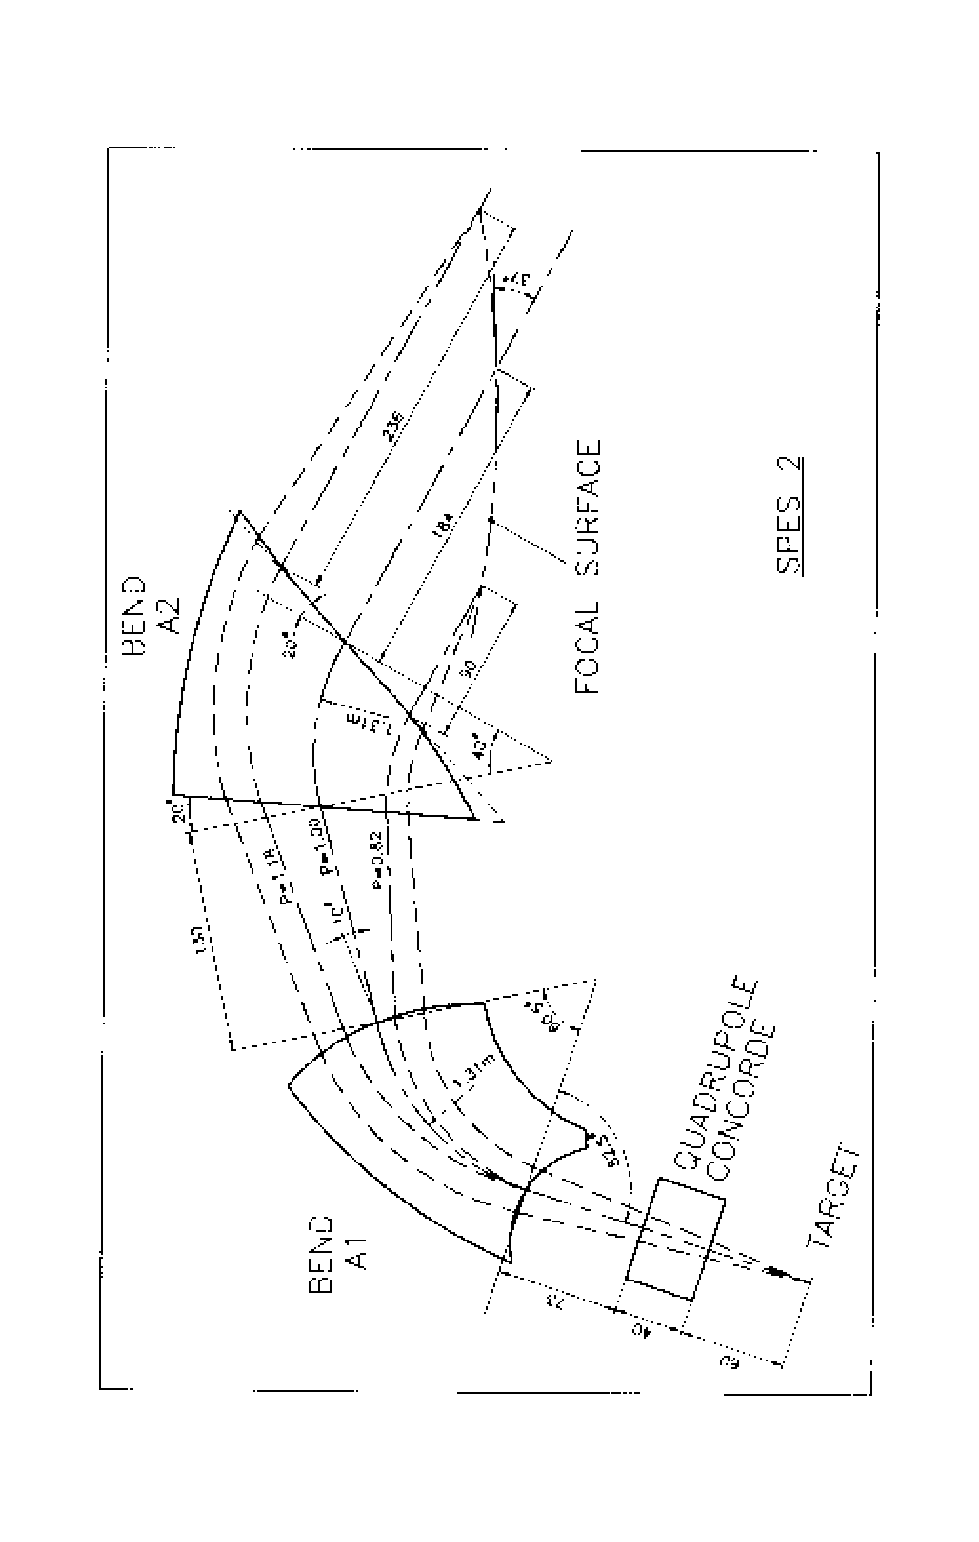
\includegraphics[height=17cm,angle=-90]{FigC1-1.eps}}
\caption{\label{figC11}Design of SPES 2.}
\end{figure}

\vfill 

\begin{tiny}
\begin{center}
\twocolumn

\noindent \textbf{\normalsize \zgoubi data file.}

\begin{alltt}
SPES2 QDD SPECTROMETER, USING FIELD MAPS; MONTE-CARLO OBJECT WITH MOMENTUM GRID.
 'MCOBJET'                                                                    1
 2335.                                REFERENCE  RIGIDITY.                      
 2                                    DISTRIBUTION  IN  GRID.                   
 10000                                NUMGER  OF  PARTICLES.                    
 1   1   1   1   1   1                UNIFORM DISTRIBUTIONS                     
 0.  0.  0.  0.  0.  1.               CENTRAL  VALUES  OF  BARS.                
 1   1   1   1   1   5                NUMBER  OF  BARS  IN  MOMENTUM.           
 0.  0.  0.  0.  0.  .001             SPACE  BETWEEN  MOMENTUM  BARS.           
 0.  50.e-3 0.  50.e-3 0.  0.         WIDTH  OF  BARS.                          
 1.  1.  1.  1.  1.  1.               SORTING CUT-OFFS (UNUSED)                 
 9   9. 9. 9. 9.                      FOR P(D) (UNUSED)                         
 186387 548728 472874                 SEEDS.                                    
  'HISTO'                                                                     2
  1   .997   1.003  80  1             HISTO  OF  D.                             
  20  'D'  1  'Q'                                                               
  'HISTO'                                                                     3
  3   -60.  60.     80  1             HISTO  OF  THETA0.                        
  20  'T'  1  'Q'                                                             
  'HISTO'                                                                     4
  5   -60.  60.     80  1             HISTO  OF  PHI0.                          
  20  'P'  1  'Q'                                                               
 'DRIFT'                                                                      5
 41.5                                                                           
 'CARTEMES'                           QUADRUPOLE  MAP.                        6
  0  0                                IC  IL.                                   
  -.96136E-3  1. 1.                   BNORM, XNorm,YNorm                        
 ++++  CONCORDE ++++                                                            
  39  23                              IX  IY.                                   
  concord.map                         field map file name, quadrupole           
  0  0 0 0                            NO  LIMIT  PLANE.                         
 2                                    IORDRE.                                   
 2.5                                  XPAS.                                     
 2 0 0 0                              KPOS.                                     
 'DRIFT'                                                                      7
 21.8                                                                           
 'CHANGREF'                           POSITIONING  OF  THE                    8
 0. 32.5 -35.6                        1-ST  BENDING.                            
 'CARTEMES'                                                                   9
  0 0                                                                           
  1.04279E-3  1. 1.                                                             
 ++++  A1 ++++                                                                  
  117  52                                                                       
  a1.map                              field map file name, first dipole         
  0  0 0 0                                                                      
 2                                                                              
 2.5                                                                            
 2 0 0 0                                                                        
 'CHANGREF'                           POSITIONING  OF  THE                   10
 0. -28.65  -27.6137                  EXIT  FRAME.                              
 'DRIFT'                                                                     11
 33.15                                                                          
 'CHANGREF'                           POSITIONING  OF  THE                   12
 0. 27.5  -19.88                      2-ND  BENDING.                            
 'CARTEMES'                                                                  13
  0 0                                                                           
  1.05778E-3  1. 1.                                                             
 ++++  A2 ++++                                                                  
  132  80                                                                       
  a2.map                              field map file name, second dipole        
  0  0 0 0                                                                      
 2                                                                              
 2.5                                                                            
 2 0 0 0                                                                        
 'CHANGREF'                           POSITIONING  OF  THE                   14
 41.  -81.  -21.945                   EXIT  FRAME.                              
 'DRIFT'                                                                     15
 3.55                                                                           
  'HISTO'                             HISTO  OF  Y :                         16
  2  -.5  2.     80  1                SHOWS  THE  RESOLUTION                    
  20  'Y'  1  'Q'                     OF  THE  SPECTROMETER.                    
 'END'                                                                       17
\end{alltt}

\newpage
\noindent \textbf{\normalsize Excerpt from \zgoubi output : histograms of initial beam coordinates.}

\begin{alltt}
**********************************************************************************************
      2  HISTO                         

                      HISTOGRAMME  DE  LA  COORDONNEE    D   
                      PARTICULES  PRIMAIRES  ET  SECONDAIRES
                      DANS  LA  FENETRE :   0.9970     /    1.003          
                      NORMALISE     

   20                                                                                                
   19                                                                                                
   18                                                                                                
   17                    D             D            D            D             D             
   16                    D             D            D            D             D             
   15                    D             D            D            D             D             
   14                    D             D            D            D             D             
   13                    D             D            D            D             D             
   12                    D             D            D            D             D             
   11                    D             D            D            D             D             
   10                    0             0            0            0             0             
    9                    D             D            D            D             D             
    8                    D             D            D            D             D             
    7                    D             D            D            D             D             
    6                    D             D            D            D             D             
    5                    D             D            D            D             D             
    4                    D             D            D            D             D             
    3                    D             D            D            D             D             
    2                    D             D            D            D             D             
    1                    D             D            D            D             D      
            123456789012345678901234567890123456789012345678901234567890123456789012345678901        
                     2         3         4         5         6         7         8         9

             
        TOTAL  COMPTAGE                 :   10000  SUR  10000
        NUMERO   DU  CANAL  MOYEN       :      51
        COMPTAGE  AU   "      "         :    2038
        VAL. PHYS. AU  "      "         :  1.000          
        RESOLUTION  PAR  CANAL          :  7.500E-0
        PARAMETRES  PHYSIQUES  DE  LA  DISTRIBUTION :
                      COMPTAGE =  10000  PARTICULES
                      MIN =  0.9980    , MAX =   1.002    , MAX-MIN =  4.0000E-03      
                      MOYENNE =   1.000          
                      SIGMA =  1.4108E-03      

 TRAJ 1 IEX,D,Y,T,Z,P,S,time :  1  0.9980  0.000 -30.24   0.000   44.63   0.0000   0.0000    

**********************************************************************************************
      3  HISTO                         
                
                      HISTOGRAMME  DE  LA  COORDONNEE  THETA 
                      PARTICULES  PRIMAIRES  ET  SECONDAIRES
                      DANS  LA  FENETRE :   -60.00     /    60.00     (MRD)
                              NORMALISE     

   20                                                                                                
   19                                                                                                
   18                                                                                                
   17                                                                      T              T          
   16                   T                             T            T              T          
   15                 T T    T      TT         T      T   T   T  T T   T       TT TT         
   14                TT T   TT   T  TTTT TT    T     TTTTTT TTTT TTTT  TT T   TTT TTT        
   13               TTTTTT TTTTTTT TTTTT TTT TTT T   TTTTTTTTTTTTTTTT TTTTT   TTTTTTTT       
   12               TTTTTTTTTTTTTTTTTTTTTTTTTTTTTTTTTTTTTTTTTTTTTTTTTTTTTTTTTTTTTTTTTT       
   11              TTTTTTTTTTTTTTTTTTTTTTTTTTTTTTTTTTTTTTTTTTTTTTTTTTTTTTTTTTTTTTTTTTT       
   10              0000000000000000000000000000000000000000000000000000000000000000000       
    9              TTTTTTTTTTTTTTTTTTTTTTTTTTTTTTTTTTTTTTTTTTTTTTTTTTTTTTTTTTTTTTTTTTT       
    8              TTTTTTTTTTTTTTTTTTTTTTTTTTTTTTTTTTTTTTTTTTTTTTTTTTTTTTTTTTTTTTTTTTT       
    7              TTTTTTTTTTTTTTTTTTTTTTTTTTTTTTTTTTTTTTTTTTTTTTTTTTTTTTTTTTTTTTTTTTT       
    6              TTTTTTTTTTTTTTTTTTTTTTTTTTTTTTTTTTTTTTTTTTTTTTTTTTTTTTTTTTTTTTTTTTT       
    5              TTTTTTTTTTTTTTTTTTTTTTTTTTTTTTTTTTTTTTTTTTTTTTTTTTTTTTTTTTTTTTTTTTT       
    4              TTTTTTTTTTTTTTTTTTTTTTTTTTTTTTTTTTTTTTTTTTTTTTTTTTTTTTTTTTTTTTTTTTT       
    3              TTTTTTTTTTTTTTTTTTTTTTTTTTTTTTTTTTTTTTTTTTTTTTTTTTTTTTTTTTTTTTTTTTT       
    2              TTTTTTTTTTTTTTTTTTTTTTTTTTTTTTTTTTTTTTTTTTTTTTTTTTTTTTTTTTTTTTTTTTT       
    1              TTTTTTTTTTTTTTTTTTTTTTTTTTTTTTTTTTTTTTTTTTTTTTTTTTTTTTTTTTTTTTTTTTT
                   
            123456789012345678901234567890123456789012345678901234567890123456789012345678901
                     2         3         4         5         6         7         8         9

              
        TOTAL  COMPTAGE                 :   10000  SUR  10000
        NUMERO   DU  CANAL  MOYEN       :      51
        COMPTAGE  AU   "      "         :     128
        VAL. PHYS. AU  "      "         :  3.331E-15 (MRD)
        RESOLUTION  PAR  CANAL          :   1.50     (MRD)
             
        PARAMETRES  PHYSIQUES  DE  LA  DISTRIBUTION :
                      COMPTAGE =  10000  PARTICULES
                      MIN =  -49.99    , MAX =   50.00    , MAX-MIN =   99.98     (MRD)
                      MOYENNE =  0.3320     (MRD)
                      SIGMA =   29.04     (MRD)

 TRAJ 1 IEX,D,Y,T,Z,P,S,time :  1  0.9980   0.000  -30.24  0.000  44.63   0.0000   0.0000    
**********************************************************************************************
\end{alltt}

\newpage
\begin{alltt}
**********************************************************************************************
      4  HISTO                         
                
                      HISTOGRAMME  DE  LA  COORDONNEE  PHI   
                      PARTICULES  PRIMAIRES  ET  SECONDAIRES
                      DANS  LA  FENETRE :   -60.00     /    60.00     (MRD)
                      NORMALISE     

   20                                                                                                
   19                                                                                        
   18                                                                                        
   17                                       PP       P   P P                                 
   16                P P P   PP             PPPPP   PPPP PPPP  PPP          PPPP P P         
   15               PPPP PPP PPP    PP   P  PPPPPP PPPPPPPPPPP PPPP PP  P  PPPPPPP P         
   14               PPPP PPP PPPP   PP PPPPPPPPPPP PPPPPPPPPPPPPPPP PPP PP PPPPPPPPP         
   13               PPPP PPPPPPPPPPPPPPPPPPPPPPPPPPPPPPPPPPPPPPPPPPPPPP PPPPPPPPPPPPP        
   12               PPPPPPPPPPPPPPPPPPPPPPPPPPPPPPPPPPPPPPPPPPPPPPPPPPPPPPPPPPPPPPPPPP       
   11              PPPPPPPPPPPPPPPPPPPPPPPPPPPPPPPPPPPPPPPPPPPPPPPPPPPPPPPPPPPPPPPPPPP       
   10              0000000000000000000000000000000000000000000000000000000000000000000       
    9              PPPPPPPPPPPPPPPPPPPPPPPPPPPPPPPPPPPPPPPPPPPPPPPPPPPPPPPPPPPPPPPPPPP       
    8              PPPPPPPPPPPPPPPPPPPPPPPPPPPPPPPPPPPPPPPPPPPPPPPPPPPPPPPPPPPPPPPPPPP       
    7              PPPPPPPPPPPPPPPPPPPPPPPPPPPPPPPPPPPPPPPPPPPPPPPPPPPPPPPPPPPPPPPPPPP       
    6              PPPPPPPPPPPPPPPPPPPPPPPPPPPPPPPPPPPPPPPPPPPPPPPPPPPPPPPPPPPPPPPPPPP       
    5              PPPPPPPPPPPPPPPPPPPPPPPPPPPPPPPPPPPPPPPPPPPPPPPPPPPPPPPPPPPPPPPPPPP       
    4              PPPPPPPPPPPPPPPPPPPPPPPPPPPPPPPPPPPPPPPPPPPPPPPPPPPPPPPPPPPPPPPPPPP       
    3              PPPPPPPPPPPPPPPPPPPPPPPPPPPPPPPPPPPPPPPPPPPPPPPPPPPPPPPPPPPPPPPPPPP       
    2              PPPPPPPPPPPPPPPPPPPPPPPPPPPPPPPPPPPPPPPPPPPPPPPPPPPPPPPPPPPPPPPPPPP       
    1              PPPPPPPPPPPPPPPPPPPPPPPPPPPPPPPPPPPPPPPPPPPPPPPPPPPPPPPPPPPPPPPPPPP       
               
            123456789012345678901234567890123456789012345678901234567890123456789012345678901
                     2         3         4         5         6         7         8         9

               
        TOTAL  COMPTAGE                 :   10000  SUR  10000
        NUMERO   DU  CANAL  MOYEN       :      51
        COMPTAGE  AU   "      "         :     163
        VAL. PHYS. AU  "      "         :  3.331E-15 (MRD)
        RESOLUTION  PAR  CANAL          :   1.50   
       
        PARAMETRES  PHYSIQUES  DE  LA  DISTRIBUTION :
                      COMPTAGE =  10000  PARTICULES
                      MIN =  -50.00    , MAX =   49.99    , MAX-MIN =   99.99     (MRD)
                      MOYENNE =  0.2838     (MRD)
                      SIGMA =   28.75     (MRD)

 TRAJ 1 IEX,D,Y,T,Z,P,S,time :  1  0.9980   0.000  -30.24  0.000  44.63   0.0000   0.0000    
**********************************************************************************************

\end{alltt}


\noindent \textbf{\normalsize Excerpt from \zgoubi output~: 
the final momentum resolution histogram at the spectrometer focal surface.}
\begin{alltt}
**********************************************************************************************
     16  HISTO       HISTO     OF      
                        
                      HISTOGRAMME  DE  LA  COORDONNEE  Y     
                      PARTICULES  PRIMAIRES  ET  SECONDAIRES
                      DANS  LA  FENETRE :  -0.5000     /    2.000     (CM) 
                      NORMALISE     

   20                                                                                                
   19                                                                                                
   18                                                                                        
   17                                              Y                                         
   16                                              Y         Y                               
   15                                              Y         Y                               
   14                                              Y         Y                               
   13                                              Y         Y                               
   12                                              Y         Y                               
   11                                              Y         Y                               
   10                                   0          0         0         0                     
    9                                   Y          Y         Y         Y                     
    8                                   Y          Y         YY        Y                     
    7                                   Y         YY         YY        YY                    
    6                       Y          YYY        YY         YY        YY                    
    5                       YY         YYY        YY         YY       YYYY                   
    4                       YY Y       YYY        YYY        YY       YYYY                   
    3                       YY YY     YYYYY       YYY       YYYY      YYYYY                  
    2                      YYYYYY     YYYYYY     YYYY       YYYYY     YYYYYY                 
    1                     YYYYYYYYYYYYYYYYYYYYYYYYYYYYYYY YYYYYYYY   YYYYYYYY         

            123456789012345678901234567890123456789012345678901234567890123456789012345678901
                     2         3         4         5         6         7         8         9

                  
        TOTAL  COMPTAGE                 :   10000  SUR  10000
        NUMERO   DU  CANAL  MOYEN       :      51
        COMPTAGE  AU   "      "         :     246
        VAL. PHYS. AU  "      "         :  0.750     (CM) 
        RESOLUTION  PAR  CANAL          :  3.125E-02 (CM) 
             
        PARAMETRES  PHYSIQUES  DE  LA  DISTRIBUTION :
                      COMPTAGE =  10000  PARTICULES
                      MIN = -0.1486    , MAX =   1.652    , MAX-MIN =   1.800     (CM) 
                      MOYENNE =  0.7576     (CM) 
                      SIGMA =  0.4621     (CM) 

 TRAJ 1 IEX,D,Y,T,Z,P,S,time :  1  0.9980 0.2475 74.43 -6.2488E-03 -6.929   697.41 0.0000    
**********************************************************************************************
\end{alltt}

\onecolumn
\end{center}
\end{tiny}

\clearpage

%%%%%%%%%%%%%%%%%%%%
%				   %
%	spes2res.tex   %
%				   %
%%%%%%%%%%%%%%%%%%%%
%\addtocounter{page}{4}  %% 3 + empty page 


%%%%%%%%%%%%%%figure%%%%%%%%%%%%%%
\section{TRANSFER MATRICES ALONG A TWO-STAGE SEPARATION KAON BEAM LINE}

\vfill

\begin{figure}[H]
%%%Figure C2-1
\centerline{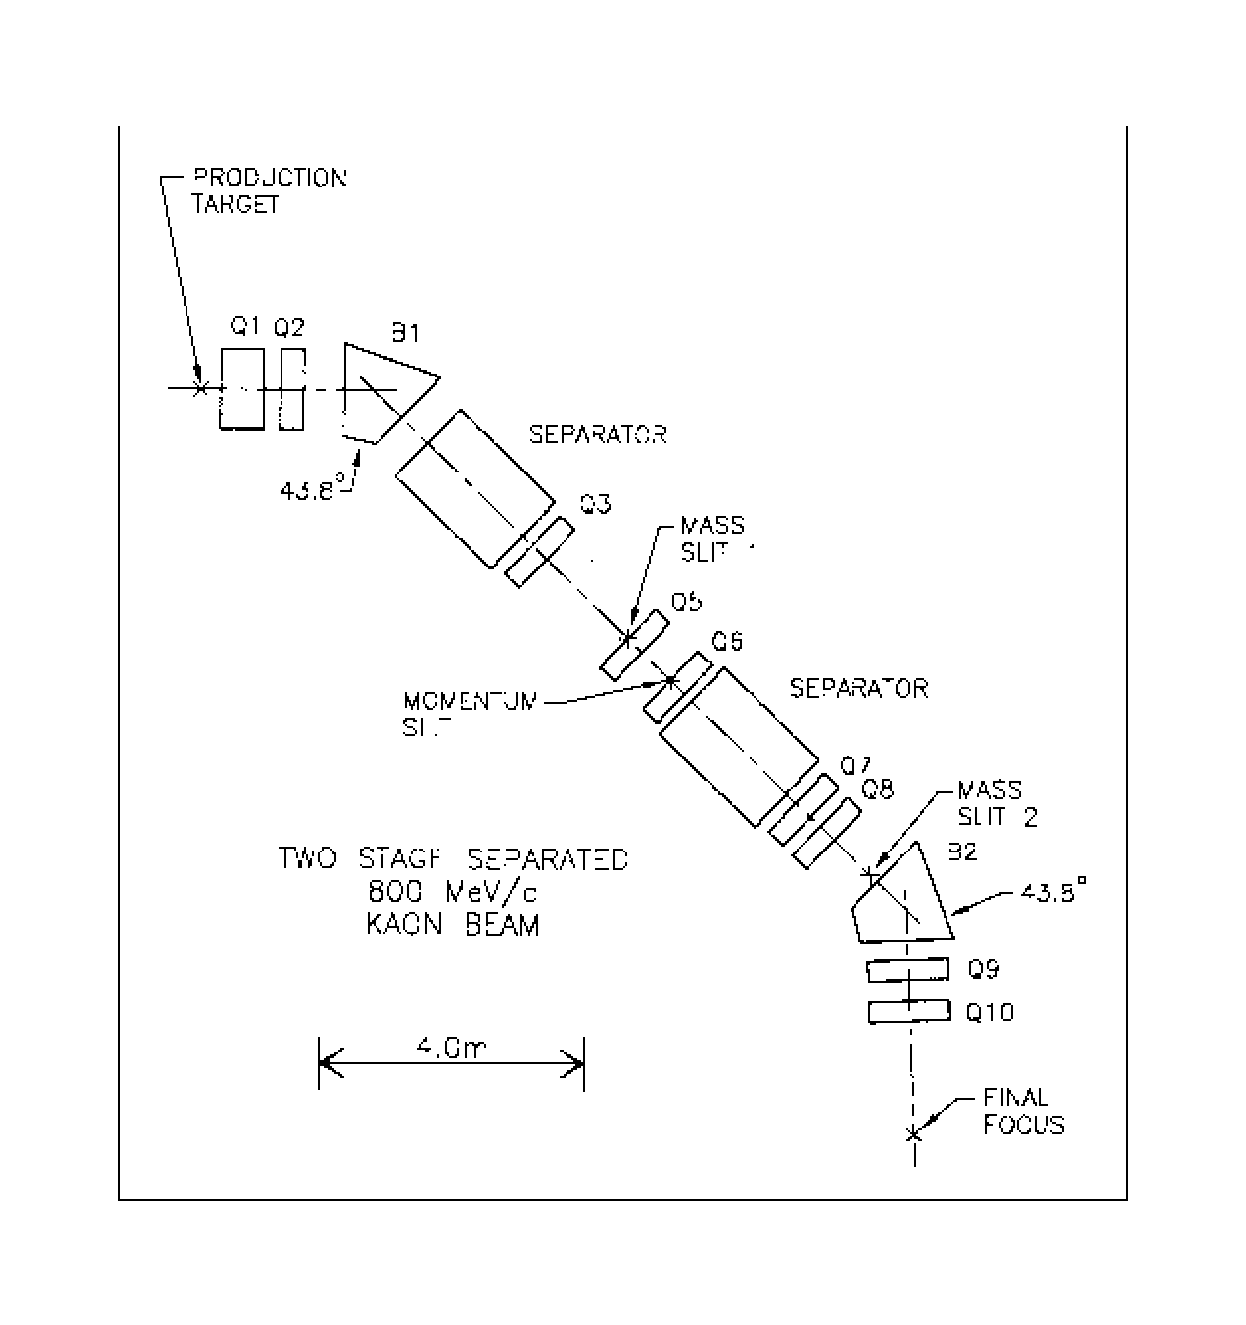
\includegraphics[width=15cm]{FigC2-1.ps}}
\vfill

\caption{\label{figC21}Design of 800 MeV/c kaon beam line.}
\end{figure}

\vfill


\begin{tiny}

\twocolumn
\noindent \textbf{\normalsize  \zgoubi data file.}
\begin{alltt}
    800 MeV/c KAON BEAM LINE. CALCULATION OF TRANSFER COEFFICIENTS.             
   'OBJET'                                                                 1
   2668.5100                             AUTOMATIC  GENERATION  OF              
   6                                     AN  OBJECT  FOR  CALCULATION           
   .1  .1  .1  .1 0.  .001      OF  THE  FIRST  ORDER  TRANSFER                 
   0. 0. 0. 0. 0. 1.                     COEFFICIENTS  WITH  'MATRIX'           
   'PARTICUL'                                                              2
    493.646 1.60217733E-19 0. 0. 0.      KAON M & Q, FOR USE IN WIEN FILTER     
   'DRIFT'                                                                 3
    35.00000                                                                    
   'QUADRUPO'                            Q1                                4
   0                                                        
     76.2  15.24  13.6                                                          
    30.  30.                                                                    
    4    0.2490   5.3630  -2.4100   0.9870   0.   0.                            
    30. 30.                                                                     
    4    0.2490   5.3630  -2.4100   0.9870   0.   0.                            
     1.1                                                                        
    1  0. 0. 0.                                                                 
   'DRIFT'                                                                 5
     25.00000                                                                   
   'QUADRUPOLE'                          Q2                                6
   0                                                        
   45.72  15.24   -11.357                                                       
    30. 30.                                                                     
    4    0.2490   5.3630  -2.4100   0.9870   0.   0.                            
    30. 30.                                                                     
    4    0.2490   5.3630  -2.4100   0.9870   0.   0.                            
     1.1                                                                        
    1  0. 0. 0.                                                                 
   'DRIFT'                                                                 7
    -1.898                                                                      
   'TOSCA'                             3-D  MAP  THE  OF  FIRST            8
    0  0                                                    BENDING  MAGNET     
   1.0313E-3  1. 1. 1.                 B, X, Y, Z normalization coefficients    
   1D map at z=0, from TOSCA                                                    
   59  39  1                                                                    
   bw6_0.map                                                                    
   0  0. 0. 0.                                                                  
   2                                                        
     1.1                                                                        
   1 0 0 0                                                                      
   'CHANGREF'                                                              9
   0.  -70.78  -43.8                                                            
  'FAISCEAU'                                                              10
    'DRIFT'                                                               11
      -49.38                                                                    
   'OCTUPOLE'                                                             12
   0                                                        
    10. 15.24  .6                                                               
    0. 0.                                                                       
    4    0.2490   5.3630  -2.4100   0.9870   0.   0.                            
    0. 0.                                                                       
    4    0.2490   5.3630  -2.4100   0.9870   0.   0.                            
    .4                                                                          
    1  0. 0. 0.                                                                 
   'SEXTUPOL'                            SX1, COMPENSATION                13
   0                                     OF  THE  Theta.Phi  ABERRATION         
   10.  15.24  2.4                       AT  VF1                                
    0.  0. 0. 0.                                                                
    4    0.2490   5.3630  -2.4100   0.9870   0.   0.                            
    0. 0.  0. 0.                                                                
    4    0.2490   5.3630  -2.4100   0.9870   0.   0.                            
     .4                                                                         
    1  0. 0. 0.                                                                 
   'DRIFT'                                                                14
     50.0                                                                       
    'WIENFILT'                           FIRST  VERTICAL  WIEN  FILTER    15
    0                                                       
   2.16  55.E5  -.0215576  2                                                    
   20. 10. 10.                                                                  
   0.2401  1.8639  -0.5572  0.3904 0. 0.                                        
   0.2401  1.8639  -0.5572  0.3904 0. 0.                                        
   20. 10. 10.                                                                  
   0.2401  1.8639  -0.5572  0.3904 0. 0.                                        
   0.2401  1.8639  -0.5572  0.3904 0. 0.                                        
   1.                                                       
  1. 0. 0. 0.                                                                   
   'DRIFT'                                                                16
     30.                                                                        
   'QUADRUPO'                            Q3                               17
   0                                                        
     45.72  15.24  -6.34                                                        
    30. 30.                                                                     
    4    0.2490   5.3630  -2.4100   0.9870   0.   0.                            
    30. 30.                                                                     
    4    0.2490   5.3630  -2.4100   0.9870   0.   0.                            
     1.1                                                                        
    1  0. 0. 0.                                                                 
   'DRIFT'                                                                18
    10.0                                                                        
   'MULTIPOL'                            SX2 + OCTU, COMPENSATION         19
   0                                     OF  THE  D.Phi  AND  D2.Phi            
   10.  15.24   0. 0. -8.  1.2  0. 0. 0. 0. 0. 0.    ABERRATIONS  AT  VF1       
    0. 0. 0. 0. 0. 0. 0. 0. 0. 0. 0. 0.                                         
    4    0.2490   5.3630  -2.4100   0.9870   0.   0.                            
    0. 0. 0. 0. 0. 0. 0. 0. 0. 0. 0. 0.                                         
    4    0.2490   5.3630  -2.4100   0.9870   0.   0.                            
   0. 0. 0. 0. 0. 0. 0. 0. 0. 0.                                                
     .4                                                                         
    1  0. 0. 0.                                                                 
   'DRIFT'                                                                20
     90.0                                                                       
   'MATRIX'                              TRANSFER  COEFFICIENTS           21
   2 0                                                                          
\end{alltt}
\newpage
\begin{alltt}
   'COLLIMA'                             FIRST  VERTICAL  FOCUS,          22
    2                                    MASS  SLIT                             
   2  14.6  .15E10  0. 0.                                                       
   'DRIFT'                                                                23
     20.0                                                                       
   'QUADRUPO'                            Q5                               24
   0                                                        
    45.72  15.24   10.93                                                        
    30. 30.                                                                     
    4    0.2490   5.3630  -2.4100   0.9870   0.   0.                            
    30. 30.                                                                     
    4    0.2490   5.3630  -2.4100   0.9870   0.   0.                            
   1.1                                                                          
    1  0. 0. 0.                                                                 
   'DRIFT'                                                                25
     10.0                                                                       
   'MULTIPOL'                            COMPENSATION  OF                 26
   0                                     ABERRATIONS  AT  VF2                   
    10.  15.24  0. 0.  0.  1.  0. 0. 0. 0. 0. 0.                                
    0. 0.  0. 0. 0. 0. 0. 0. 0. 0. 0.                                           
    4    0.2490   5.3630  -2.4100   0.9870   0.   0.                            
    0. 0.  0. 0. 0. 0. 0. 0. 0. 0. 0.                                           
    4    0.2490   5.3630  -2.4100   0.9870   0.   0.                            
   0. 0. 0. 0. 0. 0. 0. 0. 0. 0.                                                
    .4                                                                          
    1  0. 0. 0.                                                                 
   'DRIFT'                                                                27
     10.0                                                                       
   'QUADRUPO'                            Q6                               28
   0                                                        
    45.72  15.24  -11.18                                                        
    30. 30.                                                                     
    4    0.2490   5.3630  -2.4100   0.9870   0.   0.                            
    30. 30.                                                                     
    4    0.2490   5.3630  -2.4100   0.9870   0.   0.                            
     1.1                                                                        
    1  0. 0. 0.                                                                 
   'DRIFT'                                                                29
     50.0                                                                       
    'WIENFILT'                           SECOND  VERTICAL  WIEN  FILTER   30
    0                                                       
   2.16  -55.E5  .0215576  2                                                    
   20. 10. 10.                                                                  
   0.2401  1.8639  -0.5572  0.3904 0. 0.                                        
   0.2401  1.8639  -0.5572  0.3904 0. 0.                                        
   20. 10. 10.                                                                  
   0.2401  1.8639  -0.5572  0.3904 0. 0.                                        
   0.2401  1.8639  -0.5572  0.3904 0. 0.                                        
   1.                                                       
  1. 0. 0. 0.                                                                   
   'DRIFT'                                                                31
     30.0                                                                       
   'QUADRUPO'                            Q7                               32
   0                                                        
    45.72  15.24  -6.44                                                         
    30. 30.                                                                     
    4    0.2490   5.3630  -2.4100   0.9870   0.   0.                            
    30. 30.                                                                     
    4    0.2490   5.3630  -2.4100   0.9870   0.   0.                            
    1.1                                                                         
    1  0. 0. 0.                                                                 
   'DRIFT'                                                                33
     25.00000                                                                   
   'QUADRUPO'                            Q8                               34
   0                                                        
    45.72  15.24  8.085                                                         
    30. 30.                                                                     
    4    0.2490   5.3630  -2.4100   0.9870   0.   0.                            
    30. 30.                                                                     
    4    0.2490   5.3630  -2.4100   0.9870   0.   0.                            
     1.1                                                                        
    1  0. 0. 0.                                                                 
   'DRIFT'                                                               35
     40.0                                                                       
   'COLLIMA'                             SECOND  VERTICAL  FOCUS,        36
    2                                    MASS  SLIT                             
   1  17.   .2E10   0. 0.                                                       
   'MATRIX'                              TRANSFER  COEFFICIENTS          37
   2 0                                                                          
   'DRIFT'                                                               38
   -25.0                                                                        
   'DIPOLE'                              SIMULATION  OF  THE  MAP        39
    2 0 0                                OF  THE  SECOND  BENDING  MAGNET       
    150  60               (upgraded version of keyword 'AIMANT')
     18.999   0. 0. 0.                                                          
     79.3329   17.7656  140.4480   110.  170.                                   
    15. -1.                                                                     
    4  .1455   2.2670  -.6395  1.1558  0. 0.  0.                                
    0.00    21.90  1.E6 -1.E6  1.E6  1.E6                                       
    15. -1.                                                                     
    4  .1455   2.2670  -.6395  1.1558  0. 0.  0.                                
   -43.80  -21.90 -1.E6 -1.E6  1.E6 -1.E6                                       
     0                                                                          
    2                                                       
     2.5                                                                        
    2                                                       
    147.48099   -0.31007  147.48099    0.31007                                  
   'DRIFT'                                                                40
   -15.00000                                                                    
   'QUADRUPO'                            Q9                               41
   0                                                        
    35.56  12.7  -13.69  -13.91                                                 
    30.  25.4                                                                   
    4    0.2490   5.3630  -2.4100   0.9870   0.   0.                            
    30.  25.4                                                                   
    4    0.2490   5.3630  -2.4100   0.9870   0.   0.                            
     .5                                                                         
    1  0. 0. 0.                                                                 
\end{alltt}
\onecolumn
\clearpage
\begin{alltt}
   'DRIFT'                                                                42
     25.00000                                                                   
   'QUADRUPO'                            Q10                              43
   0                                                        
     35.56  12.7  11.97                                                         
    30.  25.4                                                                   
    4    0.2490   5.3630  -2.4100   0.9870   0.   0.                            
    30.  25.4                                                                   
    4    0.2490   5.3630  -2.4100   0.9870   0.   0.                            
     1.1                                                                        
    1  0. 0. 0.                                                                 
   'DRIFT'                                                                44
    200.0                                                                       
   'MATRIX'                              TRANSFER  COEFFICIENTS           45
   2 0                                   AT  THE  FINAL  FOCUS                  
   'END'                                                                  46
\end{alltt}

\noindent \textbf{\normalsize Excerpt of \zgoubi output : first and second order transfer matrices and higher 
order coefficients at the end of the line}.

\begin{alltt}
               FIRST  ORDER  COEFFICIENTS  ( MKSA ):

           3.60453       -4.453265E-02   -3.049728E-04   -1.165832E-04     0.00000       -5.229783E-02
          -2.05368        0.270335        4.700517E-05    1.763910E-05     0.00000       -9.561918E-02
          2.240965E-05   -8.687757E-07    -3.60817       -1.731805E-02     0.00000       -7.815367E-02
          1.185290E-05   -4.356398E-07    -2.05043       -0.286991         0.00000       -3.983392E-02
         -0.387557        2.313953E-02   -2.264218E-05   -8.015244E-06     1.00000        0.374917
           0.00000         0.00000         0.00000         0.00000         0.00000         1.00000

          DetY-1 =      -0.1170246601,    DetZ-1 =       0.0000034613

          R12=0 at   0.1647     m,        R34=0 at  -0.6034E-01 m

      First order sympletic conditions (expected values = 0) :
        -0.1170        3.4614E-06   -1.8207E-04    3.0973E-05    4.6007E-04   -8.0561E-05

               SECOND  ORDER  COEFFICIENTS  ( MKSA ):

   1 11   7.34       1 21  -1.78       1 31  1.399E-02   1 41  1.456E-02   1 51   0.00       1 61   36.3
   1 12  -1.78       1 22  -530.       1 32 -1.308E-03   1 42 -1.743E-03   1 52   0.00       1 62   12.3
   1 13  1.399E-02   1 23 -1.308E-03   1 33 -0.611       1 43 -0.522       1 53   0.00       1 63 -2.771E-02
   1 14  1.456E-02   1 24 -1.743E-03   1 34 -0.522       1 44  0.163       1 54   0.00       1 64 -2.211E-02
   1 15   0.00       1 25   0.00       1 35   0.00       1 45   0.00       1 55   0.00       1 65   0.00
   1 16   36.3       1 26   12.3       1 36 -2.771E-02   1 46 -2.211E-02   1 56   0.00       1 66   2.88


   2 11  -303.       2 21   3.81       2 31  3.684E-02   2 41  3.581E-02   2 51   0.00       2 61   144.
   2 12   3.81       2 22  -62.9       2 32 -5.821E-04   2 42 -1.638E-04   2 52   0.00       2 62 -0.759
   2 13  3.684E-02   2 23 -5.821E-04   2 33   1.05       2 43   1.94       2 53   0.00       2 63 -1.031E-02
   2 14  3.581E-02   2 24 -1.638E-04   2 34   1.94       2 44   6.70       2 54   0.00       2 64 -4.285E-02
   2 15   0.00       2 25   0.00       2 35   0.00       2 45   0.00       2 55   0.00       2 65   0.00
   2 16   144.       2 26 -0.759       2 36 -1.031E-02   2 46 -4.285E-02   2 56   0.00       2 66  -65.3


   3 11 -0.145       3 21  2.158E-02   3 31   20.6       3 41   86.0       3 51   0.00       3 61 -0.201
   3 12  2.158E-02   3 22   64.6       3 32   1.61       3 42  0.496       3 52   0.00       3 62  8.793E-02
   3 13   20.6       3 23   1.61       3 33  0.710       3 43  0.128       3 53   0.00       3 63   39.1
   3 14   86.0       3 24  0.496       3 34  0.128       3 44   64.8       3 54   0.00       3 64   7.17
   3 15   0.00       3 25   0.00       3 35   0.00       3 45   0.00       3 55   0.00       3 65   0.00
   3 16 -0.201       3 26  8.793E-02   3 36   39.1       3 46   7.17       3 56   0.00       3 66   1.46


   4 11 -8.254E-02   4 21  1.146E-02   4 31   10.7       4 41   47.3       4 51   0.00       4 61 -0.127
   4 12  1.146E-02   4 22   33.0       4 32  0.787       4 42  0.157       4 52   0.00       4 62  3.566E-02
   4 13   10.7       4 23  0.787       4 33  0.365       4 43  6.774E-02   4 53   0.00       4 63   17.5
   4 14   47.3       4 24  0.157       4 34  6.774E-02   4 44   33.1       4 54   0.00       4 64   1.05
   4 15   0.00       4 25   0.00       4 35   0.00       4 45   0.00       4 55   0.00       4 65   0.00
   4 16 -0.127       4 26  3.566E-02   4 36   17.5       4 46   1.05       4 56   0.00       4 66  0.715


   5 11   568.       5 21  -7.67       5 31 -5.970E-02   5 41 -5.682E-02   5 51   0.00       5 61  -251.
   5 12  -7.67       5 22   225.       5 32  1.283E-03   5 42  6.947E-04   5 52   0.00       5 62   2.77
   5 13 -5.970E-02   5 23  1.283E-03   5 33   19.2       5 43   10.2       5 53   0.00       5 63  0.215
   5 14 -5.682E-02   5 24  6.947E-04   5 34   10.2       5 44   1.59       5 54   0.00       5 64  0.129
   5 15   0.00       5 25   0.00       5 35   0.00       5 45   0.00       5 55   0.00       5 65   0.00
   5 16  -251.       5 26   2.77       5 36  0.215       5 46  0.129       5 56   0.00       5 66   112.

               HIGHER  ORDER  COEFFICIENTS  ( MKSA ):

           Y/Y3            5784.8
           Y/T3           9.40037E+05
           Y/Z3           0.70673
           Y/P3           0.42104

           T/Y3           -18607.
           T/T3           1.04607E+05
           T/Z3          -0.10234
           T/P3           5.25793E-02

           Z/Y3            32.161
           Z/T3            18.425
           Z/Z3           -872.50
           Z/P3           -785.20

           P/Y3            15.460
           P/T3            7.5264
           P/Z3           -409.98
           P/P3           -389.15
\end{alltt}

\end{tiny}


 \clearpage

%%%%%%%%%%%%%%%%%%%
%				  %
%            kaonres.tex	  %
%				  %
%%%%%%%%%%%%%%%%%%%
%\addtocounter{page}{8}  %% 7 + empty page

%\newpage
%\eject
%\newpage
%%%%%%%%%%%%%%figure%%%%%%%%%%%%%%
\section{IN-FLIGHT DECAY IN SPES 3}
%\centerline{\textbf{EXAMPLE 3: SPES 3}}
%\addcontentsline{toc}{section}{\numberline{3}IN-FLIGHT DECAY IN SPES 3}
\vfill

\begin{figure}[H]
%%%Figure C3-1
\centerline{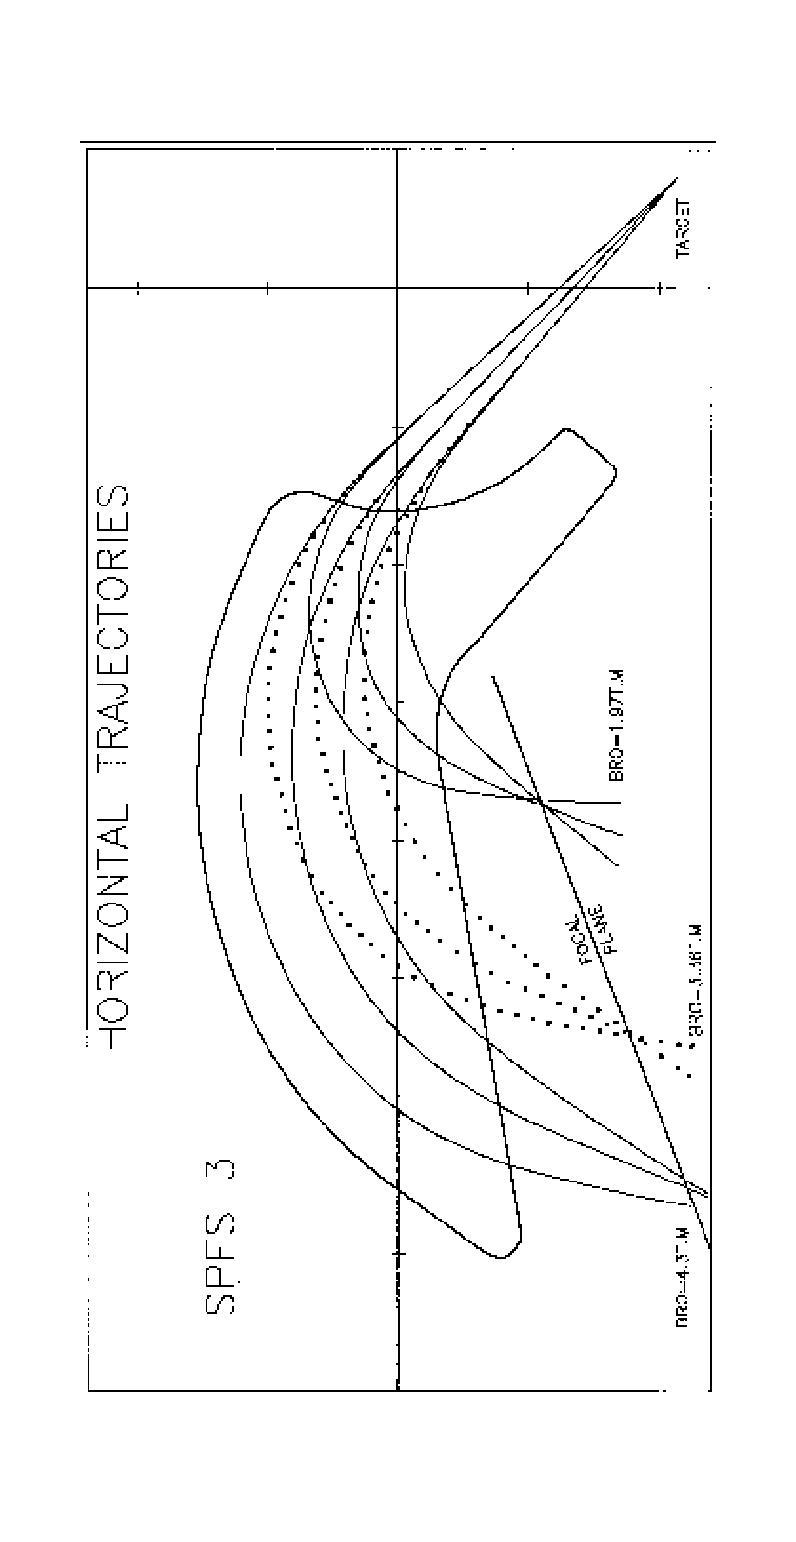
\includegraphics[height=17cm,angle=-90]{FigC3-1.eps}}
\caption{\label{figC31}Design of SPES 3.}
\end{figure}

\vfill
\newpage

\noindent {\textbf  \normalsize \zgoubi data file}
\footnotesize
\begin{alltt}
  SIMULATION  OF  PION  IN-FLIGHT  DECAY  IN  SPES3                             
  'MCOBJET'                                                              1      
  3360.                                REFERENCE  RIGIDITY (PION).              
  1                                    DISTRIBUTION  IN  WINDOW.                
  200                                  BUNCHES  OF  200  PARTICLES.             
  1     1       1     1      1    1    UNIFORM DISTRIBUTION                     
  0.    0.      0.    0.     0.   1.   CENTRAL  VALUES  OF  BARS.               
  .5e-2 50.e-3 .5e-2  50.e-3 0.  0.4   WIDTH  OF  BARS.                         
  1     1       1     1      1    1    CUT-OFFS (UNUSED)                        
  9   9. 9. 9. 9.                      UNUSED.                                  
  186387 548728 472874                 SEEDS.                                   
  'PARTICUL'                                                             2      
  139.6000 0. 0. 26.03E-9 0.           PION MASS AND LIFE TIME                  
  'MCDESINT'                                                             3      
  105.66   0.                          PION -> MUON + NEUTRINODECAY             
  136928 768370 548375                                                          
  'ESL'                                                                  4      
  77.3627                                                                       
  'CHAMBR'                             STOPS  ABERRANT  MUONS.           5      
  1                                                                             
  1   100. 10. 245.  0.                                                         
  'DIPOLE'                                                               6      
  2 0 0                                                                         
  180  130                                                                      
  30     0. 0. 0.                                                               
  80.   33.     208.5  140.  350.                                               
  46. -1.                                                                       
  4. .14552 5.21405 -3.38307 14.0629 0. 0. 0.                                   
   15.   0.      -65.  0.    0.  -65.                                           
  46. -1.                                                                       
  4. .14552 5.21405 -3.38307 14.0629 0. 0. 0.                                   
  -15.  69.       85.  0.    1.E6  1.E6                                         
  0                                                                             
  2                                                                             
  4.                                                                            
  2                                                                             
  164.755 .479966 233.554 -.057963                                              
  'CHAMBR'                                                               7      
  2                                                                             
  1   100. 10. 245.  0.                                                         
  'CHANGREF'                          TILT  ANGLE  OF                    8      
  0.   0.   -49.                      FOCAL  PLANE.                             
  'HISTO'                             TOTAL  SPECTRUM (PION + MUON).     9      
  2  -170.  130.  60  1                                                         
  20  'Y'  1  'Q'                                                               
  'HISTO'                             PION  SPATIAL  SPECTRUM           10      
  2  -170.  130.  60  2               AT  FOCAL  PLANE.                         
  20  'P'  1  'P'                                                               
  'HISTO'                             MUON  SPATIAL  SPECTRUM           11      
  2  -170.  130.  60  3               AT  FOCAL  PLANE.                         
  20  'y'  1  'S'                                                               
  'HISTO'                             MUON  MOMENTUM  SPECTRUM          12      
  1    .2   1.7   60  3               AT  FOCAL  PLANE.                         
  20  'd'  1  'S'                                                               
  'REBELOTE'                          (49+1)  RUNS =  CALCULATION  OF   13      
  49  0.1  0                          (49+1)*200  TRAJECTORIES.                 
  'END'                                                                 14      
\end{alltt}



\clearpage
\tiny
\twocolumn
\noindent \textbf{\normalsize Excerpt of \zgoubi output : histograms of primary and secondary particles at focal surface of SPES3.}

\begin{alltt}
*******************************************************************************************
      9  HISTO     TOTAL     SPECTRUM

                              HISTOGRAMME  DE  LA  COORDONNEE  Y    
                              PARTICULES  PRIMAIRES  ET  SECONDAIRES
                              DANS  LA  FENETRE :  -1.7000E+02 /   1.3000E+02 (CM) 
                              NORMALISE     

   20                                                                                      
   19                                                                                      
   18                                                                                      
   17                                             Y     YY        Y  Y      Y              
   16                                           Y YYYYY YY YYY  Y YY Y Y  YYYY             
   15                                           Y YYYYY YYYYYYYYYYYYYY YYYYYYYY YY         
   14                                         YYYYYYYYY YYYYYYYYYYYYYYYYYYYYYYYYYYY        
   13                                         YYYYYYYYY YYYYYYYYYYYYYYYYYYYYYYYYYYY        
   12                                         YYYYYYYYYYYYYYYYYYYYYYYYYYYYYYYYYYYYY        
   11                                         YYYYYYYYYYYYYYYYYYYYYYYYYYYYYYYYYYYYY        
   10                                         0000000000000000000000000000000000000        
    9                                         YYYYYYYYYYYYYYYYYYYYYYYYYYYYYYYYYYYYY        
    8                                         YYYYYYYYYYYYYYYYYYYYYYYYYYYYYYYYYYYYY        
    7                                         YYYYYYYYYYYYYYYYYYYYYYYYYYYYYYYYYYYYY        
    6                                         YYYYYYYYYYYYYYYYYYYYYYYYYYYYYYYYYYYYY        
    5                                         YYYYYYYYYYYYYYYYYYYYYYYYYYYYYYYYYYYYY        
    4                                         YYYYYYYYYYYYYYYYYYYYYYYYYYYYYYYYYYYYY        
    3                                         YYYYYYYYYYYYYYYYYYYYYYYYYYYYYYYYYYYYY        
    2                                        YYYYYYYYYYYYYYYYYYYYYYYYYYYYYYYYYYYYYY        
    1                                        YYYYYYYYYYYYYYYYYYYYYYYYYYYYYYYYYYYYYYY       

                              1234567890123456789012345678901234567890123456789012345678901
                                       3         4         5         6         7         8


                TOTAL  COMPTAGE                 :    9887  SUR  10000
                NUMERO   DU  CANAL  MOYEN       :      55
                COMPTAGE  AU   "      "         :     281
                VAL. PHYS. AU  "      "         :  0.000E+00 (CM) 
                RESOLUTION  PAR  CANAL          :  5.000E+00 (CM) 

                PARAMETRES  PHYSIQUES  DE  LA  DISTRIBUTION :
                              COMPTAGE =   9887  PARTICULES
                              MIN = -1.6687E+02, MAX = 9.4131E+01, MAX-MIN = 2.6100E+02(CM) 
                              MOYENNE = -9.2496E-01 (CM) 
                              SIGMA =  5.3583E+01 (CM) 

*******************************************************************************************
     10  HISTO     PION      SPATIAL 

                              HISTOGRAMME  DE  LA  COORDONNEE  Y    
                              PARTICULES  PRIMAIRES                 
                              DANS  LA  FENETRE :  -1.7000E+02 /   1.3000E+02 (CM) 
                              NORMALISE     

   20                                                                                      
   19                                                                                      
   18                                                   P                                  
   17                                             P     PP        P  P      P              
   16                                             PP    PP PPP  P PP P P  PPPPP            
   15                                           P PPPPP PPPPPPPPPPPPPPPPPPPPPPP PP         
   14                                         PPPPPPPPP PPPPPPPPPPPPPPPPPPPPPPPPPPP        
   13                                         PPPPPPPPPPPPPPPPPPPPPPPPPPPPPPPPPPPPP        
   12                                         PPPPPPPPPPPPPPPPPPPPPPPPPPPPPPPPPPPPP        
   11                                         PPPPPPPPPPPPPPPPPPPPPPPPPPPPPPPPPPPPP        
   10                                         0000000000000000000000000000000000000        
    9                                         PPPPPPPPPPPPPPPPPPPPPPPPPPPPPPPPPPPPP        
    8                                         PPPPPPPPPPPPPPPPPPPPPPPPPPPPPPPPPPPPP        
    7                                         PPPPPPPPPPPPPPPPPPPPPPPPPPPPPPPPPPPPP        
    6                                         PPPPPPPPPPPPPPPPPPPPPPPPPPPPPPPPPPPPP        
    5                                         PPPPPPPPPPPPPPPPPPPPPPPPPPPPPPPPPPPPP        
    4                                         PPPPPPPPPPPPPPPPPPPPPPPPPPPPPPPPPPPPP        
    3                                         PPPPPPPPPPPPPPPPPPPPPPPPPPPPPPPPPPPPP        
    2                                        PPPPPPPPPPPPPPPPPPPPPPPPPPPPPPPPPPPPPP        
    1                                        PPPPPPPPPPPPPPPPPPPPPPPPPPPPPPPPPPPPPPP       

                              1234567890123456789012345678901234567890123456789012345678901
                                       3         4         5         6         7         8


                TOTAL  COMPTAGE                 :    9282  SUR  10000
                NUMERO   DU  CANAL  MOYEN       :      55
                COMPTAGE  AU   "      "         :     264
                VAL. PHYS. AU  "      "         :  0.000E+00 (CM) 
                RESOLUTION  PAR  CANAL          :  5.000E+00 (CM) 

                PARAMETRES  PHYSIQUES  DE  LA  DISTRIBUTION :
                              COMPTAGE =   9282  PARTICULES
                              MIN= -9.5838E+01, MAX = 9.3504E+01, MAX-MIN = 1.8934E+02 (CM) 
                              MOYENNE =  4.9971E-01 (CM) 
                              SIGMA =  5.3215E+01 (CM) 

*******************************************************************************************

\end{alltt}

\newpage

\begin{alltt}






*******************************************************************************************
     11  HISTO     MUON      SPATIAL 

                              HISTOGRAMME  DE  LA  COORDONNEE  Y    
                              PARTICULES  SECONDAIRES               
                              DANS  LA  FENETRE :  -1.7000E+02 /   1.3000E+02 (CM) 
                              NORMALISE     

   20                                                                                      
   19                                                                                      
   18                                               y                                      
   17                                               y        yy                            
   16                                               y        yy                            
   15                                           y   y y     yyy   y                        
   14                                           y   y y  y  yyyy  y                        
   13                                           y   yyy  yy yyyy  y                        
   12                                          yy y yyy yyy yyyyy y    y                   
   11                                         yyy y yyy yyy yyyyy y    y   y               
   10                                         000 0 000 000000000000   0   00              
    9                                         yyyyy yyy yyyyyyyyyyyy y y   yy              
    8                                        yyyyyyyyyy yyyyyyyyyyyyyy y   yy              
    7                                      yyyyyyyyyyyyyyyyyyyyyyyyyyy y  yyy              
    6                                      yyyyyyyyyyyyyyyyyyyyyyyyyyy y yyyy              
    5                                   y  yyyyyyyyyyyyyyyyyyyyyyyyyyyyyyyyyy yyy          
    4                                   y  yyyyyyyyyyyyyyyyyyyyyyyyyyyyyyyyyyyyyy          
    3                                   y  yyyyyyyyyyyyyyyyyyyyyyyyyyyyyyyyyyyyyyy         
    2                             yy   yy  yyyyyyyyyyyyyyyyyyyyyyyyyyyyyyyyyyyyyyy         
    1                             yy  yyyyyyyyyyyyyyyyyyyyyyyyyyyyyyyyyyyyyyyyyyyyy        

                              1234567890123456789012345678901234567890123456789012345678901
                                       3         4         5         6         7         8


                TOTAL  COMPTAGE                 :     605  SUR  10000
                NUMERO   DU  CANAL  MOYEN       :      50
                COMPTAGE  AU   "      "         :      14
                VAL. PHYS. AU  "      "         : -2.500E+01 (CM) 
                RESOLUTION  PAR  CANAL          :  5.000E+00 (CM) 

                PARAMETRES  PHYSIQUES  DE  LA  DISTRIBUTION :
                              COMPTAGE =    605  PARTICULES
                              MIN= -1.6687E+02, MAX = 9.4131E+01, MAX-MIN = 2.6100E+02 (CM) 
                              MOYENNE = -2.2782E+01 (CM) 
                              SIGMA =  5.4452E+01 (CM) 

*******************************************************************************************
     12  HISTO     MUON      MOMENTUM

                              HISTOGRAMME  DE  LA  COORDONNEE    D  
                              PARTICULES  SECONDAIRES               
                              DANS  LA  FENETRE :   2.0000E-01 /   1.7000E+00      
                              NORMALISE     

   20                                                                                      
   19                                                                                      
   18                                           d   d                                      
   17                                           d   d                                      
   16                                           d   dd                                     
   15                                          dd   dd                                     
   14                                         ddd d dd                                     
   13                                         ddd d dd     dd                              
   12                                         ddd d dd     dd                              
   11                                         ddd d ddd d  dd                              
   10                                        0000 0 000 0  00                              
    9                                       ddddd ddddd dd dd                              
    8                                      ddddddddddddddd ddddd                           
    7                                      dddddddddddddddddddddd                          
    6                                     dddddddddddddddddddddddd ddd                     
    5                                    dddddddddddddddddddddddddddddd                    
    4                                  ddddddddddddddddddddddddddddddddd                   
    3                                  ddddddddddddddddddddddddddddddddd  d                
    2                                 ddddddddddddddddddddddddddddddddddd dddd             
    1                                 dddddddddddddddddddddddddddddddddddddddd             

                              1234567890123456789012345678901234567890123456789012345678901
                                       3         4         5         6         7         8


                TOTAL  COMPTAGE                 :     605  SUR  10000
                NUMERO   DU  CANAL  MOYEN       :      46
                COMPTAGE  AU   "      "         :      16
                VAL. PHYS. AU  "      "         :  8.250E-01      
                RESOLUTION  PAR  CANAL          :  2.500E-02      

                PARAMETRES  PHYSIQUES  DE  LA  DISTRIBUTION :
                              COMPTAGE =    605  PARTICULES
                              MIN =  3.7184E-01, MAX =  1.3837E+00, MAX-MIN =  1.0119E+00      
                              MOYENNE =  8.1693E-01      
                              SIGMA =  2.2849E-01      

*******************************************************************************************
\end{alltt}
\onecolumn

\normalsize

 \clearpage

%%%%%%%%%%%%%%%%%%%%
%				   %
%	spes3res.tex   %
%				   %
%%%%%%%%%%%%%%%%%%%%
%\addtocounter{page}{6} %% 5+ empty page 

%%%%%%%%%%%%%%figure%%%%%%%%%%%%%%
%\centerline{\textbf{EXAMPLE 4: BACKWARD RAY-TRACING}}
%\addcontentsline{toc}{section}{\numberline{4}BACKWARD RAY-TRACING}
%\vfill

%\begin{figure}[H]
%%%%Figure C4-1
%\centerline{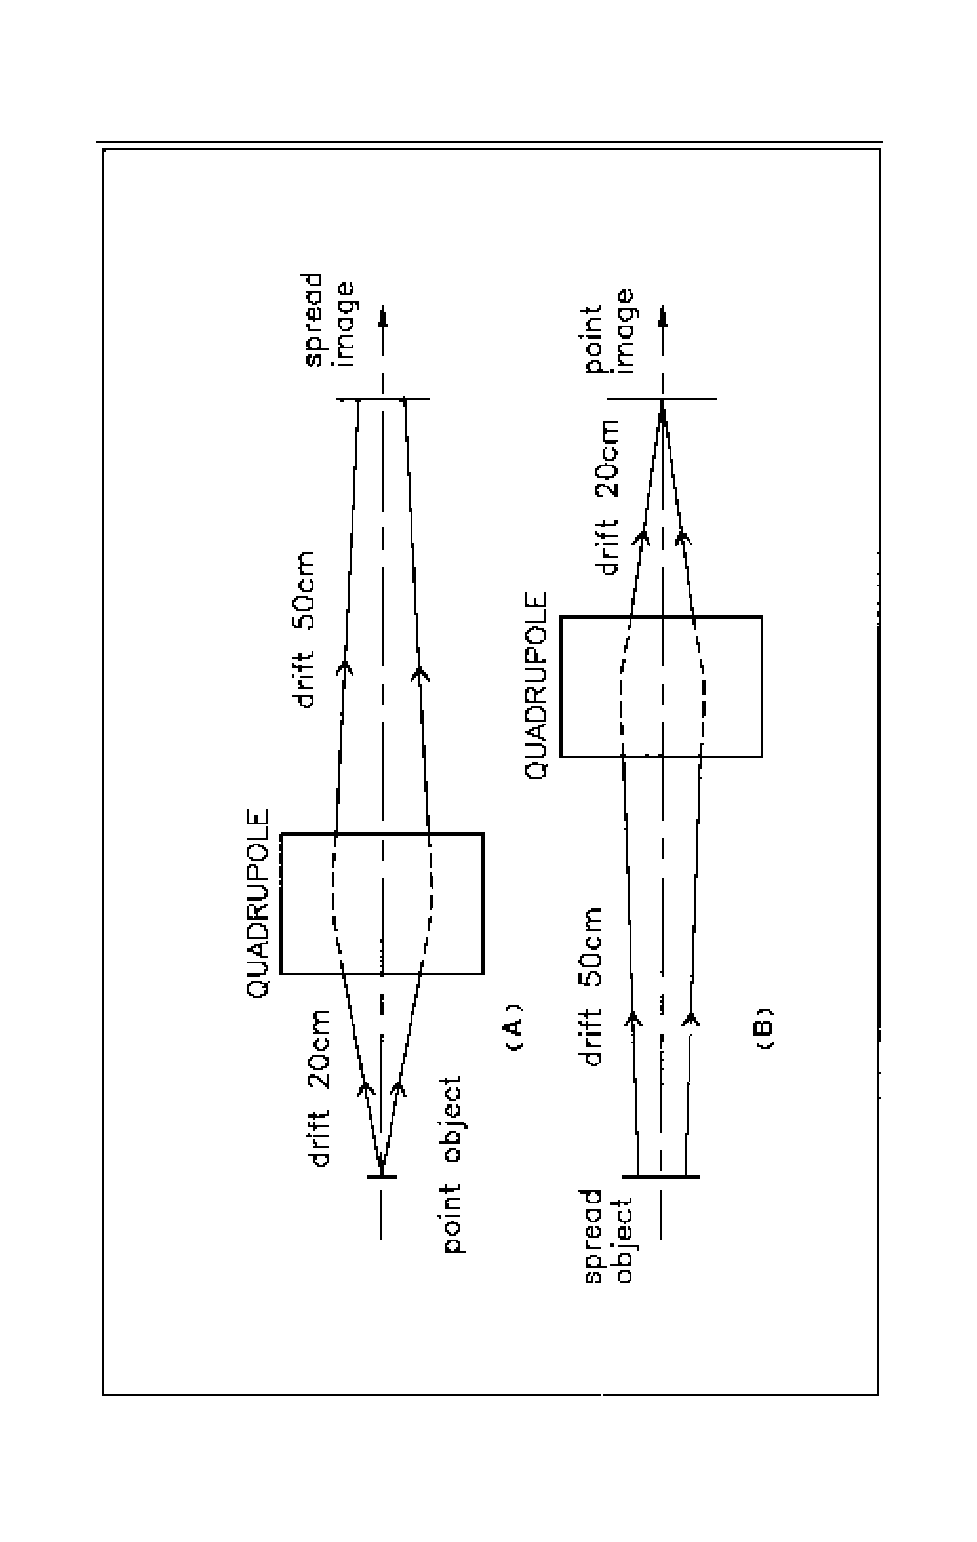
\includegraphics[width=13cm,angle=-90]{Fig36.ps}}
%\hangcaption[FigC41]{\label{figC41}A. Regular forward ray-tracing.\\
%B. Same  structure, with backward ray-tracing from image to object.} 
%\end{figure}
%\vfill
% \clearpage

%%%%%%%%%%%%%%%%%%%%
%%				  %
%%	backres.tex	  %
%%				  %
%%%%%%%%%%%%%%%%%%%%
%\addtocounter{page}{2}


 %%%%%%%%%%%%%%figure%%%%%%%%%%%%%%
\section{USE OF THE FITTING PROCEDURE}
%\centerline{\textbf{EXAMPLE 4: THE FITTING PROCEDURE}}
%\addcontentsline{toc}{section}{\numberline{4}USE OF THE FITTING PROCEDURE}
\vfill

\begin{figure}[H]
%%%Figure C5-1
\centerline{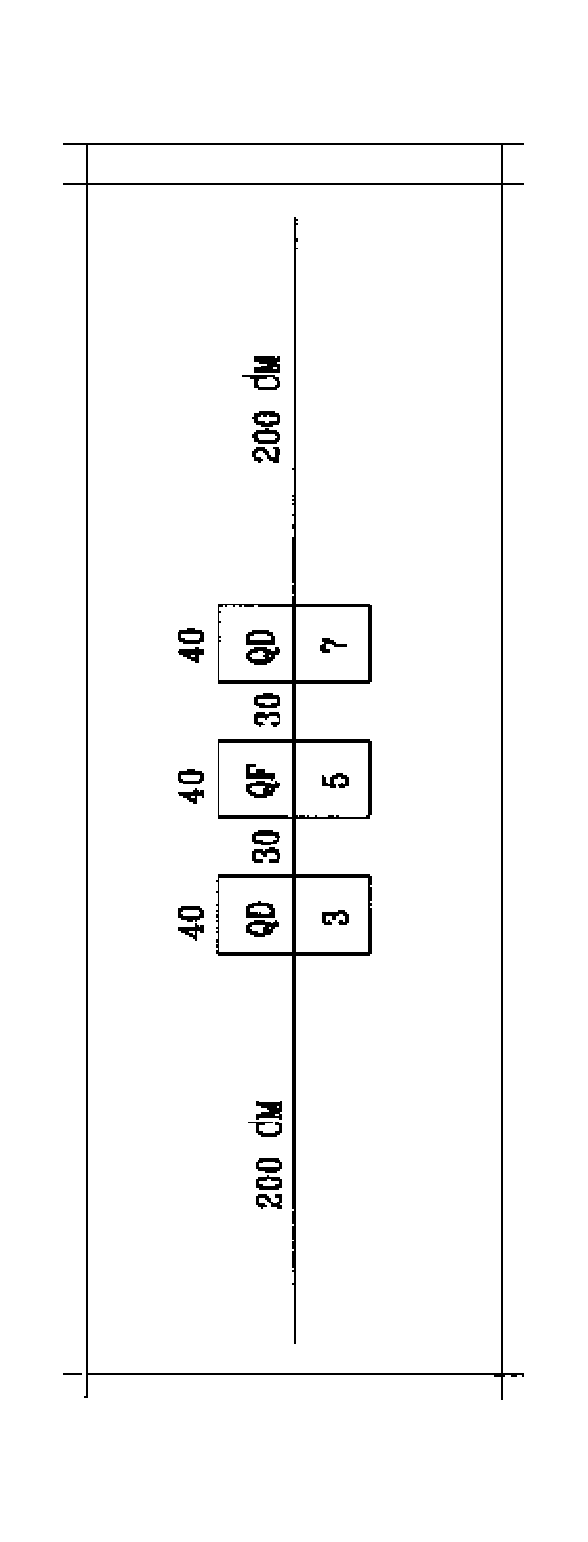
\includegraphics[height=15cm,angle=-90]{FigC5-1.ps}}
{\setlength{\captionwidth}{14cm}
\hangcaption[FigC51]{\label{figC51}Vary B in all quadrupoles, for fitting of the 
transfer coefficients $ R_{12} $ and $ R_{34} $ at the end of the line. The 
first and last quadrupoles are coupled so as to present the same 
value of B.}  }
\end{figure}

\vfill 

\begin{center}
\noindent \textbf{ \zgoubi data file.}
\begin{tiny}
\begin{alltt}
                                                MATCHING A SYMMETRIC QUADRUPOLE TRIPLET                          
                                                'OBJET'                                                                1      
                                                2501.73                        750MeV/c PROTONS                               
                                                5                              11 PARTICLES FOR USE OF MATRIX                 
                                                2.  2.  2.   2.  0. .001                                                      
                                                0.  0.  0.   0.  0.  1.                                                       
                                                'ESL   '                                                               2      
                                                200.                                                                          
                                                'QUADRUPO'    3                                                        3      
                                                 0                                                                            
                                                40.  15.  -7.                                                                 
                                                0.  0.                                                                        
                                                6  .1122 6.2671 -1.4982 3.5882 -2.1209 1.723                                  
                                                0.   0.                                                                       
                                                6  .1122 6.2671 -1.4982 3.5882 -2.1209 1.723                                  
                                                5.                                                                            
                                                1 0. 0. 0.                                                                    
                                                'ESL'                                                                  4      
                                                30.                                                                           
                                                'QUADRUPO'     5                                                       5      
                                                 0                                                                            
                                                40.  15.  3.                                                                  
                                                0.  0.                                                                        
                                                6  .1122 6.2671 -1.4982 3.5882 -2.1209 1.723                                  
                                                0.   0.                                                                       
                                                6  .1122 6.2671 -1.4982 3.5882 -2.1209 1.723                                  
                                                5.                                                                            
                                                1 0. 0. 0.                                                                    
                                                'ESL'                                                                  6      
                                                30.                                                                           
                                                'QUADRUPO'      7                                                      7      
                                                 0                                                                            
                                                40.  15.  -7.                                                                 
                                                0.  0.                                                                        
                                                6  .1122 6.2671 -1.4982 3.5882 -2.1209 1.723                                  
                                                0.   0.                                                                       
                                                6  .1122 6.2671 -1.4982 3.5882 -2.1209 1.723                                  
                                                5.                                                                            
                                                1 0. 0. 0.                                                                                                                 
                                                'ESL'                                                                  8      
                                                200.                                                                          
                                                'MATRIX'                                                               9      
                                                1  0                                                                          
                                               'FIT'               VARY B IN QUADS FOR FIT OF R12 AND R34             10      
                                                2                  FIRST ORDER TRANSFER COEFFICIENTS                          
                                                3  12 7.12  2.     SYMMETRIC TRIPLET => QUADS #1 AND #3 ARE COUPLED           
                                                5  12  0.   2.     PARAMETER #12 OF ELEMENTS #3, 5 AND 7 IS FIELD VALUE       
                                                2                                                                             
                                                1  1 2 8 16.6 1.   FIRST CONSTRAINT: R12=16.6, AFTER ELEMENT #8 (LAST DRIF    
                                                1  3 4 8 -.88 1.   SECOND CONSTRAINT: R34=-.88                                
                                               'END'                                                                  11      
\end{alltt}
\end{tiny}

\clearpage

\twocolumn
\noindent \textbf{\normalsize Excerpt of \zgoubi output : 
 first order transfer matrices prior to and after fitting.
}

\begin{scriptsize}
\begin{alltt}
*******************************************************************************************
 TRANSFER MATRIX WITH STARTING  CONDITIONS :


                  MATRICE  DE  TRANSFERT  ORDRE  1  ( MKSA )

         5.43642  17.02625   0.00000   0.00000   0.00000   0.00000
         1.67617   5.43442   0.00000   0.00000   0.00000   0.00000
         0.00000   0.00000  -1.27013  -0.97430   0.00000   0.00000
         0.00000   0.00000  -0.62915  -1.27004   0.00000   0.00000
         0.00000   0.00000   0.00000   0.00000   1.00000   0.00000
         0.00000   0.00000   0.00000   0.00000   0.00000   1.00000


*******************************************************************************************

STATE OF VARIABLES  AFTER  MATCHING :


          VARIABLE  ELEMENT    3,  PRMTR #12 :
               COUPLED  WITH  ELEMENT    7,  PRMTR #12

 STATUS OF VARIABLES
 LMNT  VAR  PARAM  MINIMUM     INITIAL        FINAL        MAXIMUM     STEP
   3    1    12  -8.384E+00  -6.986E+00  -6.98648097E+00 -5.590E+00  2.424E-16
   5    2    12   2.585E+00   3.230E+00   3.22956371E+00  3.877E+00  1.208E-16
 STATUS OF CONSTRAINTS
 TYPE  I   J  LMNT#      DESIRED         WEIGHT        REACHED        KI2
   1   1   2     8      1.6600E+01     1.0000E+00    1.6600000E+01   8.2185E-02
   1   3   4     8     -8.8000E-01     1.0000E+00   -8.8000000E-01   9.1781E-01

*******************************************************************************************

FINAL RUN, WITH NEW VARIABLES :

      9  MATRIX    9                 

           Frame for MATRIX calculation moved by :
            XC =    0.000 CM , YC =    0.000  CM ,   A =  0.00000 DEG  ( = 0.000000 RD )
            Path length of particle #1 :    580.0000 m



                  MATRICE  DE  TRANSFERT  ORDRE  1  ( MKSA )

         5.272531  16.600000   0.000000   0.000000   0.000000   0.000000
         1.614433   5.272531   0.000000   0.000000   0.000000   0.000000
         0.000000   0.000000  -1.244124  -0.880000   0.000000   0.000000
         0.000000   0.000000  -0.622552  -1.244124   0.000000   0.000000
         0.000000   0.000000   0.000000   0.000000   1.000000   0.000000
         0.000000   0.000000   0.000000   0.000000   0.000000   1.000000

      Determinants  :        DetY-1 = -.0000011112
                             DetZ-1 = -.0000000156

       R12=0  at       -3.1484  meters
       R34=0  at       -0.7073  meters

      First order sympletic conditions (expected values = 0) :
        -1.1112E-06   -1.5616E-08    0.0000E+00    0.0000E+00    0.0000E+00    0.0000E+00
*******************************************************************************************
\end{alltt}
\end{scriptsize}
\onecolumn

\end{center}

 \clearpage

%%%%%%%%%%%%%%%%%%
%				 %
%	fitres.tex	 %
%				 %
%%%%%%%%%%%%%%%%%%
%\addtocounter{page}{2}  %% 2
 %%%%%%%%%%%%%%figure%%%%%%%%%%%%%%
\section{MULTITURN SPIN TRACKING IN SATURNE 3 GeV SYNCHROTRON}
%\centerline{\textbf{EXAMPLE 5: MULTITURN TRACKING AND SPIN RESONANCE
%CROSSING IN SATURNE }
%\addcontentsline{toc}{section}{\numberline{5}MULTITURN SPIN TRACKING 
%IN SATURNE}}

%\vfill
\begin{figure}[H]
%%%%FigureC6-2 
\begin{center}

%\includegraphics[height=11cm,angle=-90]{FigC6-2.ps}

\vspace{-5mm}

\mbox{
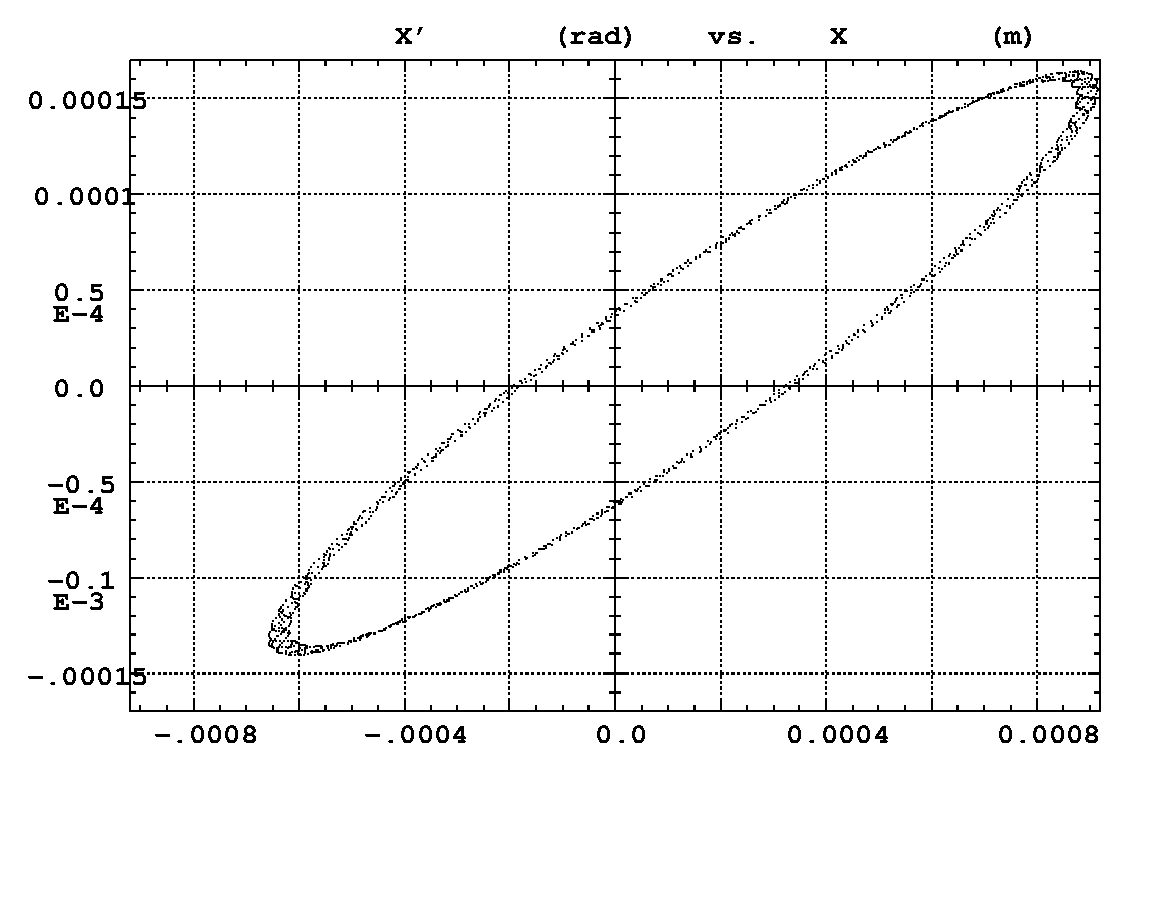
\includegraphics[height=5.8cm]{FigC6-2a.ps}
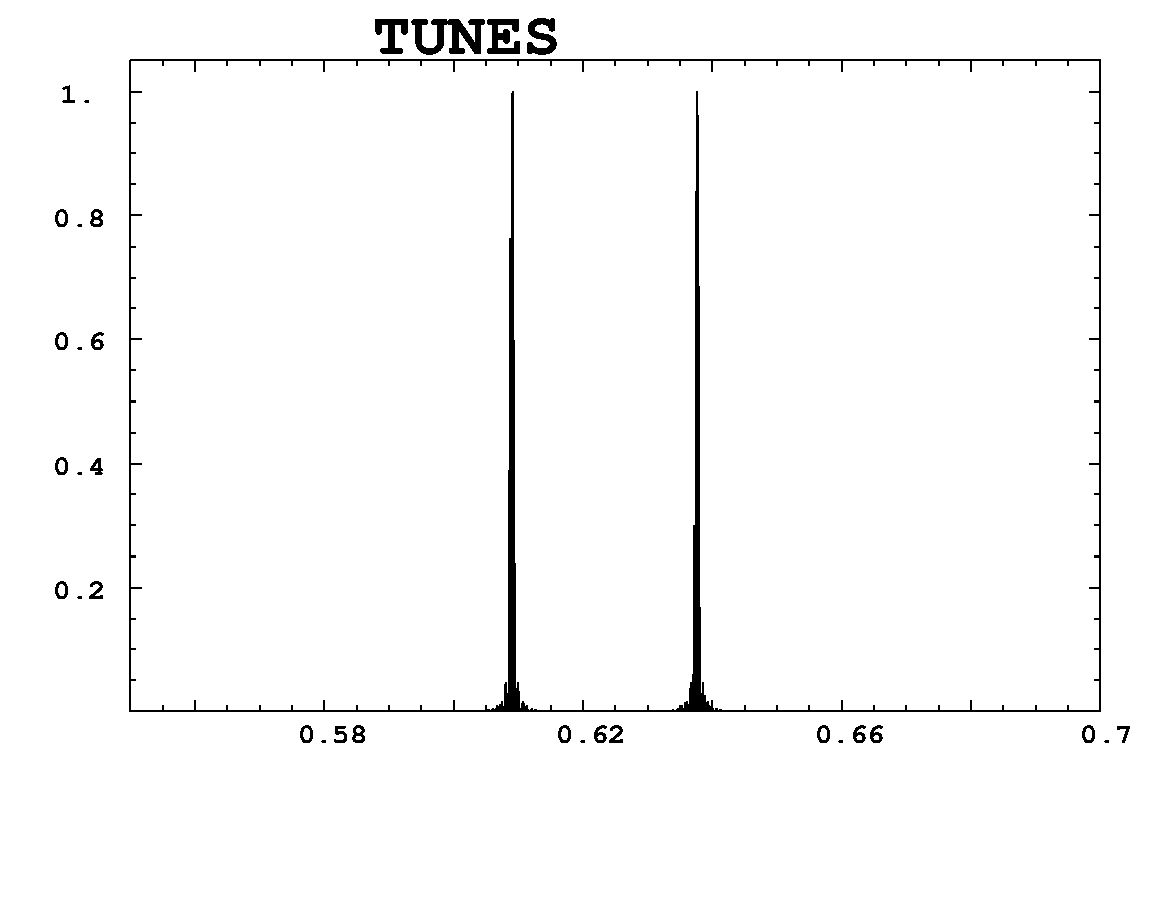
\includegraphics[height=5.8cm]{FigC6-2b.ps} 
}

\vspace{-10mm}
\mbox{
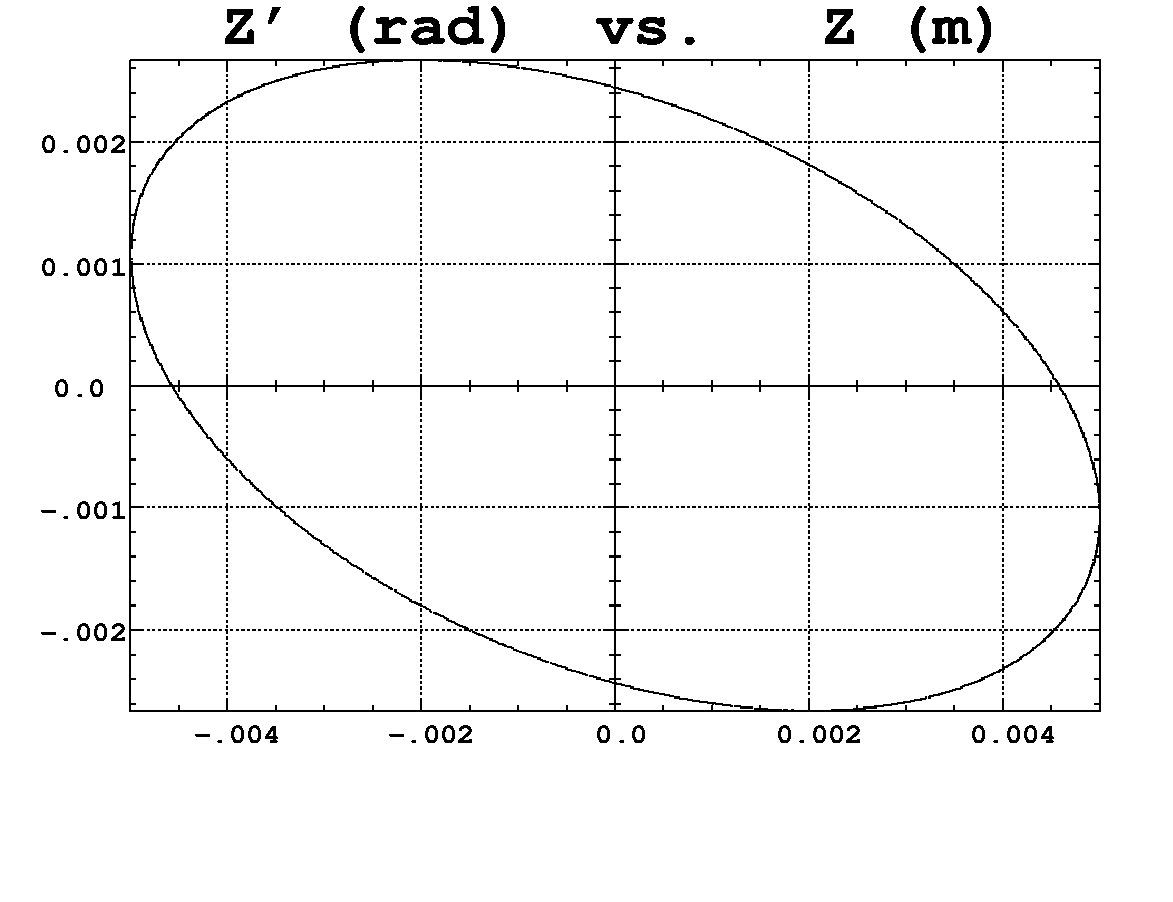
\includegraphics[height=5.8cm]{FigC6-2c.ps}
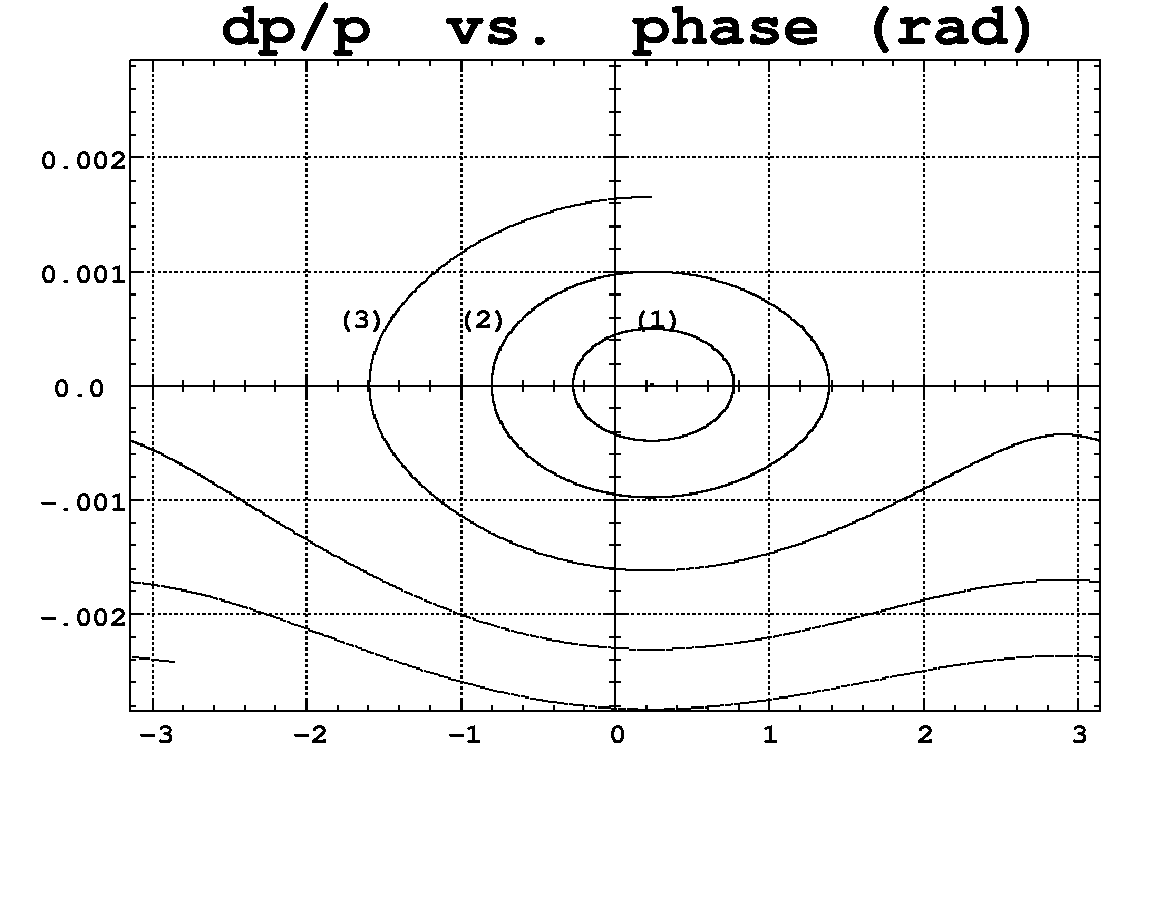
\includegraphics[height=5.8cm]{FigC6-2d.ps}
}

\vspace{-15mm}
\caption[FigC62]{\label{figC62} \small
Tracking  over 3000 turns. These 
simulations exhibit the first order parameters and 
motions as produced by the multiturn\index{multiturn} ray-tracing. \\
\textbf{(A)} Horizontal phase-space: the particle has been launched near to 
the  closed orbit (the fine structure is due to $Y-Z$ coupling induced by bends fringe fields, also 
responsible of the off-centering of the local closed orbit - at ellipse center). \\
\textbf{(B)} Vertical phase-space: the particle has been launched with 
$Z_0=4.58\ 10^{-3} $ m, $ Z^{\prime}_ 0=0$.  A least-square fit by 
$ \gamma_ZZ^2+2\alpha_ ZZZ^\prime +\beta_ ZZ^{^\prime 2}=\varepsilon_ Z/\pi $ 
 yields $ \beta_ Z=2.055 $~m, $ \alpha_Z=0.444$, $ \gamma_Z=0.582$~m$ ^{-1} $,  $ \varepsilon_Z/\pi =12\ 10^{-6}$~m.rad
 in agreement with  matrix calculations. \\
\textbf{(C)} Fractional tune numbers obtained by Fourier analysis 
for $ \varepsilon_ Y/\pi =\varepsilon_ Z/\pi \simeq 12\ 10^{-6} $~m.rad: 
%%%%%%%%%%%%% old guide  $\nu_Y=0.6375$,  $ \nu_ Z=0.6088 $ (the integer part is 3 for both). 
$\nu_ Y=0.63795$,  $ \nu_ Z=0.60912 $ (the integer part is 3 for both). \\
\textbf{(D)} Longitudinal phase-space (DP, phase): articles with initial momentum dispersion 
of $ 5\ 10^{-4} $ (1), $ 10^{-3} $ (2),
1.65~$ 10^{-3}$ (3) (out of acceptance), are accelerated at 1405 eV/turn 
($\dot  B=2.1 $ T/s); analytical calculations give accordingly 
momentum acceptance of 1.65~10$^{-3} $. }
\end{center}

\end{figure}

\vfill
%%%%%%%%%%%%%%figure%%%%%%%%%%%%%%
\vspace{-1cm}

\begin{figure}[H]
%%%FigureC6-4
\centerline{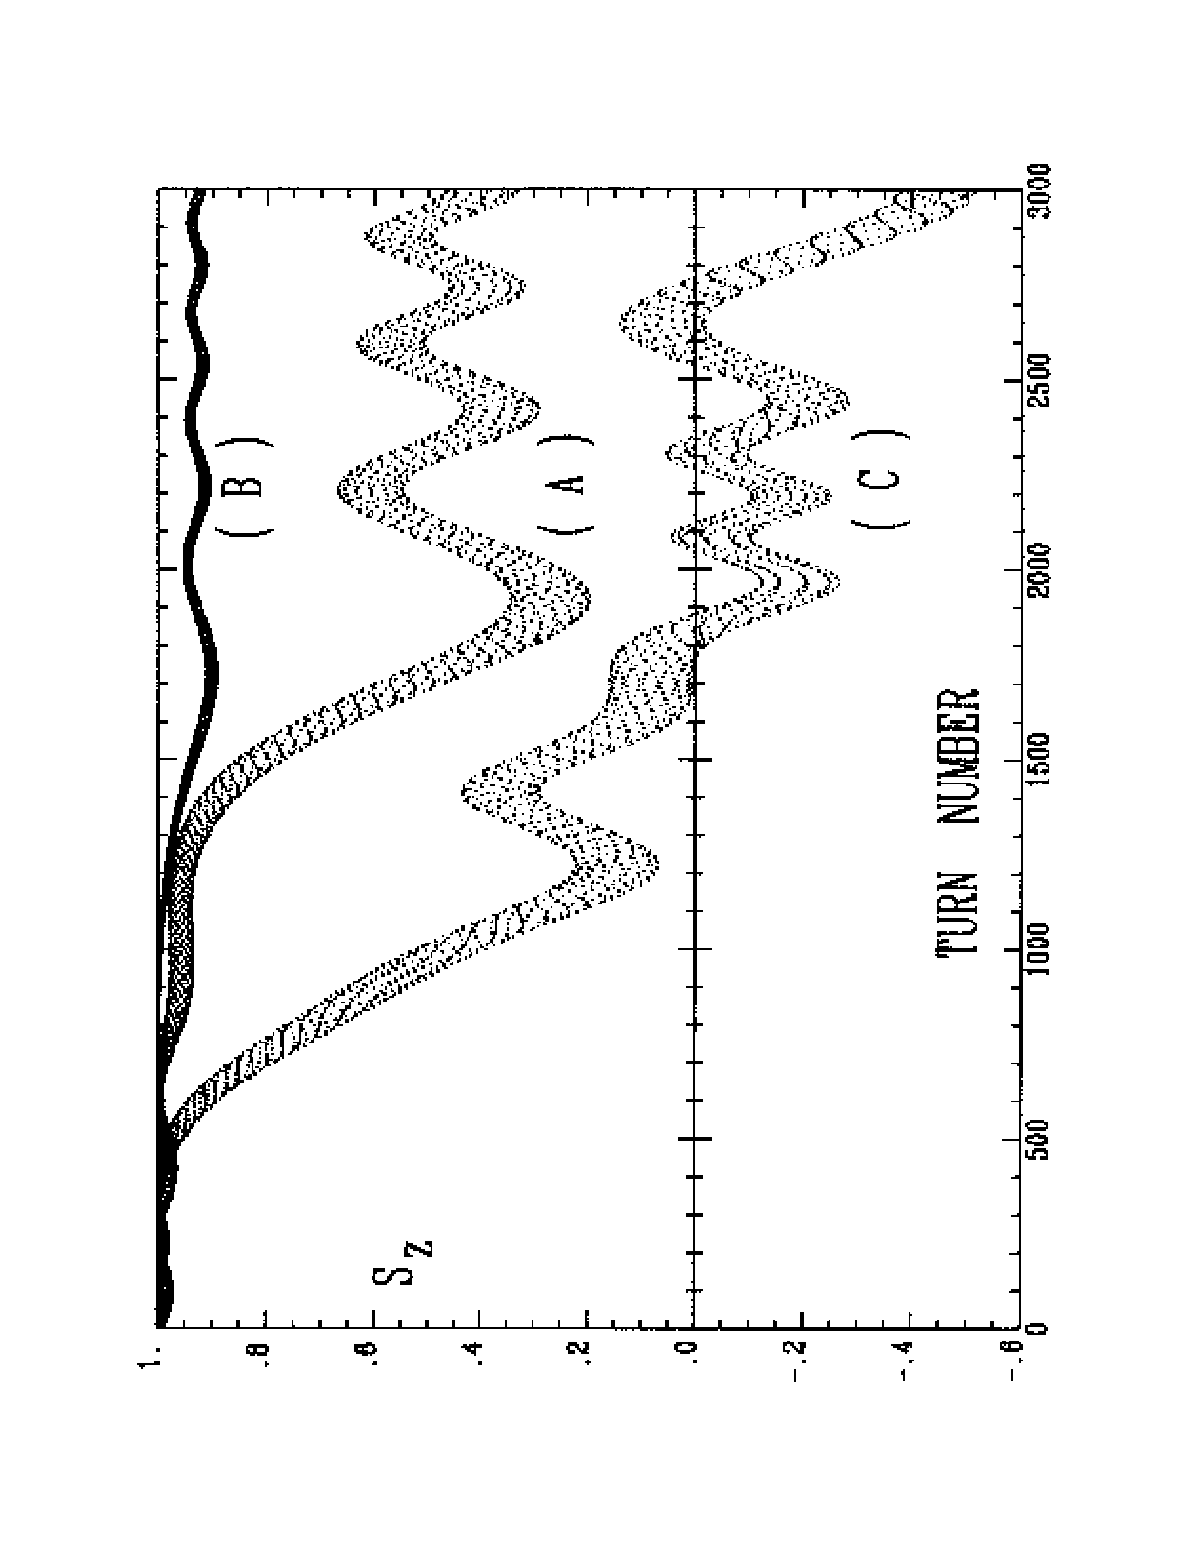
\includegraphics[height=8cm,angle=-90]{FigC6-4.ps}}
\vspace{-.2cm}
\caption[FigC64]{\label{figC64} \small
Crossing of	$ \gamma G=7-\nu_ Z	$, at $	\dot  B=2.1	$~T/s. \\
\textbf{(A)}	$ \varepsilon_ Z/\pi =12.2\	10^{-6}	$~m.rad. The strength of the resonance is
$\mid \varepsilon \mid =3.3~10^{-4}	$.
As expected	from the Froissart-Stora formula the asymptotic	polarization is	about
0.44. \\
\textbf{(B)}	The	emittance is now $ \varepsilon_	Z/\pi =1.2\	10^{-6}	$~m.rad;
comparison with	(A)	shows that $\mid \varepsilon \mid$ is proportional to
$ \protect\sqrt{\varepsilon_Z}	$.	\\
\textbf{(C)}	Crossing of	this resonance for a particle having a momentum	dispersion of
$ 10^{-3} $.}
\end{figure}

\clearpage

\twocolumn

\noindent \textbf{\normalsize  \zgoubi data file (begining and end).}
\begin{tiny}
\begin{alltt}
  SATURNE. CROSSING GammaG=7-NUz, NUz=3.60877(perturbed) 
  'OBJET' 
  5015.388                                         834.04 MeV, proton                       
  2
   4  1
 6.2E-02     6.5E-02   .458  0.  0.  1.00    'o'   EpsilonY/pi ~ 0. (Closed orbit)
 0.356       0.379     .458  0.  0.  1.0005  '1'
 0.647       0.689     .458  0.  0.  1.001   '2'
 1.024       1.09      .458  0.  0.  1.0016  '3'
 1 1 1 1
 'SCALING'
 1  4                  
   MULTIPOL 
   2                                    CROSSING GammaG=7-Nuz+/-14E, E=3.3E-4    
   5015.388E-3  5034.391E-3             AT 2.1 T/s, IN 3442 MACHINE TURNS,       
   1            3442                    FROM 834.041 TO  838.877 MeV             
   QUADRUPO
   2                                                                             
   5015.388E-3  5034.391E-3                                                      
   1            3442                                                             
   BEND                                                                          
   2                                                                             
   5015.388E-3  5034.391E-3                                                      
   1            3442                                                             
   CAVITE                                                                        
   2                                                                             
   1.           1.00378894              RELATIVE CHANGE OF SYNCRHONOUS RIGIDITY  
   1            3442                                                             
 'PARTICUL'
  938.2723  1.6021892E-19  1.7928474 0. 0.  
 'SPNTRK'
 3  
 'QUADRUPO'                 QP  1                                        5      
   0                                                                             
  46.723  10.  .763695                             .763695  = FIELD FOR BORO=1 T.m          
  0.  0.                                                                         
  6  .1122 6.2671 -1.4982 3.5882 -2.1209 1.723                                   
  0.  0.                                                                         
  6  .1122 6.2671 -1.4982 3.5882 -2.1209 1.723                                   
  #30|50|30 Quad                                                                          
  1 0. 0. 0.                                                                     
  'ESL'                      SD  2                                        6      
  71.6256                                                                        
   'BEND'                    DIP 3 4 3                                    7      
    0                                                                            
   247.30039  0.  1.57776                                             
     20. 8. .04276056667                                               
   4 .2401  1.8639  -.5572  .3904 0. 0. 0.                                       
     20. 8. .04276056667         20.  8.                                                 
   4 .2401  1.8639  -.5572  .3904 0. 0. 0.                                       
   #30|120|30   bend\                                                                         
   3 0. 0. 0. -.1963495408                                                                  
  'ESL'                      SD  2                                        8      
  71.6256                                                                        
  'MULTIPOL'                 QP  5                                        9      
   0                                                                             
  48.6273  10. 0. -.77319 0. 0. .0 .0   0. 0. 0. 0.      -.77319=-.765533+QUAD DEFECT    
  0.  0. 0. 0. 0. .0 .0  0. 0. 0. 0.                     FOR EXCITING THE DEPOLARIZING   
  6  .1122 6.2671 -1.4982 3.5882 -2.1209 1.723           RESONNANCE.                     
  0.  0. 0. 0. 0.  0. 0.   0. 0. 0. 0.                                                    
  6  .1122 6.2671 -1.4982 3.5882 -2.1209 1.723                                   
  0. 0. 0. 0. 0. 0.   0. 0. 0. 0.                                                               
  #30|50|30 Quad                                                                          
  1 0. 0. 0.                                                                     
 'ESL'                      SD  2                                        10      
  71.6256                                                                        
   'BEND'                    DIP 3 4 3                                   11      
    0                                                                            
   247.30039  0.  1.57776                                             
     20. 8. .04276056667                                               
   4 .2401  1.8639  -.5572  .3904 0. 0. 0.                                       
     20. 8. .04276056667         20.  8.                                                 
   4 .2401  1.8639  -.5572  .3904 0. 0. 0.                                       
   #30|120|30   bend\                                                                         
   3 0. 0. 0. -.1963495408                                                                  
  'ESL'                      SD  2                                       12      
  71.6256                                                                        
  'QUADRUPO'                 QP  1                                       13      
   0                                                                             
  46.723  10.  .763695                                                           
  0.  0.                                                                         
  6  .1122 6.2671 -1.4982 3.5882 -2.1209 1.723                                   
  0.  0.                                                                         
  6  .1122 6.2671 -1.4982 3.5882 -2.1209 1.723                                   
  #30|50|30 Quad                                                                          
  1 0. 0. 0.                                                                     
  'ESL'                      SD  2                                       14      
  71.6256                                                                        
   'BEND'                    DIP 3 4 3                                   15      
    0                                                                            
   247.30039  0.  1.57776                                             
     20. 8. .04276056667                                               
   4 .2401  1.8639  -.5572  .3904 0. 0. 0.                                       
     20. 8. .04276056667         20.  8.                                                 
   4 .2401  1.8639  -.5572  .3904 0. 0. 0.                                       
   #30|120|30   bend\                                                                         
   3 0. 0. 0. -.1963495408                                                                  
  'ESL'                      SD  2                                       16      
  71.6256                                                                        
  'MULTIPOL'                 QP  5                                       17      
   0                                                                             
  48.6273  10.  0.  -.765533 0. 0. 0. 0.   0. 0. 0. 0.                                          
  0.  0. 0. 0. 0.  0. 0.    0. 0. 0. 0.                                                         
  6  .1122 6.2671 -1.4982 3.5882 -2.1209 1.723                                   
  0.  0. 0. 0. 0.  0. 0.    0. 0. 0. 0.                                                         
  6  .1122 6.2671 -1.4982 3.5882 -2.1209 1.723                                   
  0. 0. 0. 0. 0. 0.   0. 0. 0. 0.                                                               
  #30|50|30 Quad                                                                          
  1 0. 0. 0.                                                                     
\end{alltt}
\newpage
\begin{alltt}
  'ESL'                      SD  2                                       18      
  71.6256                                                                        
   'BEND'                    DIP 3 4 3                                   19      
    0                                                                            
   247.30039  0.  1.57776                                             
     20. 8. .04276056667                                               
   4 .2401  1.8639  -.5572  .3904 0. 0. 0.                                       
     20. 8. .04276056667         20.  8.                                                 
   4 .2401  1.8639  -.5572  .3904 0. 0. 0.                                       
   #30|120|30   bend\                                                                         
   3 0. 0. 0. -.1963495408                                                                  
  'ESL'                      SD  2                                       20      
  71.6256                                                                        
  'QUADRUPO'                 QP  1                                       21      
   0                                                                             
  46.723  10.  .763695                                                           
  0.  0.                                                                         
  6  .1122 6.2671 -1.4982 3.5882 -2.1209 1.723                                   
  0.  0.                                                                         
  6  .1122 6.2671 -1.4982 3.5882 -2.1209 1.723                                   
  #30|50|30 Quad                                                                          
  1 0. 0. 0.                                                                     
 'ESL'                                                                   22      
 392.148                                                                         
  'MULTIPOL'                 QP  5                                       23      
   0                                                                             
  48.6273  10.  0.  -.765533 0. 0. 0. 0.   0. 0. 0. 0.                                          
  0.  0. 0. 0. 0.  0. 0.   0. 0. 0. 0.                                                          
  6  .1122 6.2671 -1.4982 3.5882 -2.1209 1.723                                   
  0.  0. 0. 0. 0.  0. 0.   0. 0. 0. 0.                                                          
  6  .1122 6.2671 -1.4982 3.5882 -2.1209 1.723                                   
  0. 0. 0. 0. 0. 0.    0. 0. 0. 0.                                                              
  #30|50|30 Quad                                                                          
  1 0. 0. 0.                                                                     
 'ESL'                                                                   24      
 392.148                                                                         
  'QUADRUPO'                 QP  1                                       25      
   0                                                                             
  46.723  10.  .763695  
  0.  0.                                                                         
  6  .1122 6.2671 -1.4982 3.5882 -2.1209 1.723                                   
  0.  0.                                                                         
  6  .1122 6.2671 -1.4982 3.5882 -2.1209 1.723                                   
  #30|50|30 Quad                                                                          
  1 0. 0. 0.                                                                     
  'ESL'                      SD  2                                       26      
  71.6256                                                                        
   'BEND'                    DIP 3 4 3                                   27      
    0                                                                            
   247.30039  0.  1.57776                                             
     20. 8. .04276056667                                               
   4 .2401  1.8639  -.5572  .3904 0. 0. 0.                                       
     20. 8. .04276056667         20.  8.                                                 
   4 .2401  1.8639  -.5572  .3904 0. 0. 0.                                       
   #30|120|30   bend\                                                                         
   3 0. 0. 0. -.1963495408                                                                  
  'ESL'                      SD  2                                       28      
  71.6256                                                                        
  'MULTIPOL'                 QP  5                                       29      
   0                                                                             
  48.6273  10.  0. -.765533  0. 0. 0. 0.   0. 0. 0. 0.                                          
  0.  0. 0. 0. 0.  0. 0.    0. 0. 0. 0.                                                         
  6  .1122 6.2671 -1.4982 3.5882 -2.1209 1.723                                   
  0.  0. 0. 0. 0.  0. 0.   0. 0. 0. 0.                                                          
  6  .1122 6.2671 -1.4982 3.5882 -2.1209 1.723                                   
  0. 0. 0. 0. 0. 0.    0. 0. 0. 0.                                                              
  #30|50|30 Quad                                                                          
  1 0. 0. 0.                                                                     
 'ESL'                      SD  2                                        30      
  71.6256                                                                        
   'BEND'                    DIP 3 4 3                                   31      
    0                                                                            
   247.30039  0.  1.57776                                             
     20. 8. .04276056667                                               
   4 .2401  1.8639  -.5572  .3904 0. 0. 0.                                       
     20. 8. .04276056667         20.  8.                                                 
   4 .2401  1.8639  -.5572  .3904 0. 0. 0.                                       
   #30|120|30   bend\                                                                         
   3 0. 0. 0. -.1963495408                                                                  

  ;;;;;;;;;;;;;;;;;;;;;;;;;;;;;;;;;;;;;;;;;;;;;;;;;;;;;;;

  'ESL'                                                                  84 
  392.148                                                                                 
  'CAVITE'                                                               85      
   1                                                                             
  105.5556848673   3.                                                                  
  6000.      0.                   SIN(phis) = .234162, dE=1.40497 keV/Turn.      
 'FAISCNL'                                                               86      
  b_zgoubi.fai                                                                     
  'SPNPRNL'                                                              87      
  zgoubi.spn                                                                     
  'SPNPRT'                                                               88      
  'REBELOTE'                                                             90      
  2999  0.1 99                     TOTAL NUMBER OF TURNS = 3000                  
 'END'                                                                   91     
\end{alltt}
\end{tiny}

\clearpage

\onecolumn


%%%%%%%%%%%%%%%%%%%%%%
%					 %
%	saturneres.tex	 %
%					 %
%%%%%%%%%%%%%%%%%%%%%%
%\addtocounter{page}{4}  %% 3 + empty page

%%%%%%%%%%%%%%figure%%%%%%%%%%%%%%
\section{MICRO-BEAM FOCUSING WITH ELECTROMAGNETIC QUADRUPOLES}
%\centerline{\textbf{EXAMPLE 6: ACHROMATIC MICRO-BEAM LINE }}
%\addcontentsline{toc}{section}{\numberline{6}MICRO-BEAM FOCUSING WITH 
%ELECTROMAGNETIC QUADRUPOLES}
\vfill

\begin{figure}[H]
  %%%FigureC7-1 
  \centerline{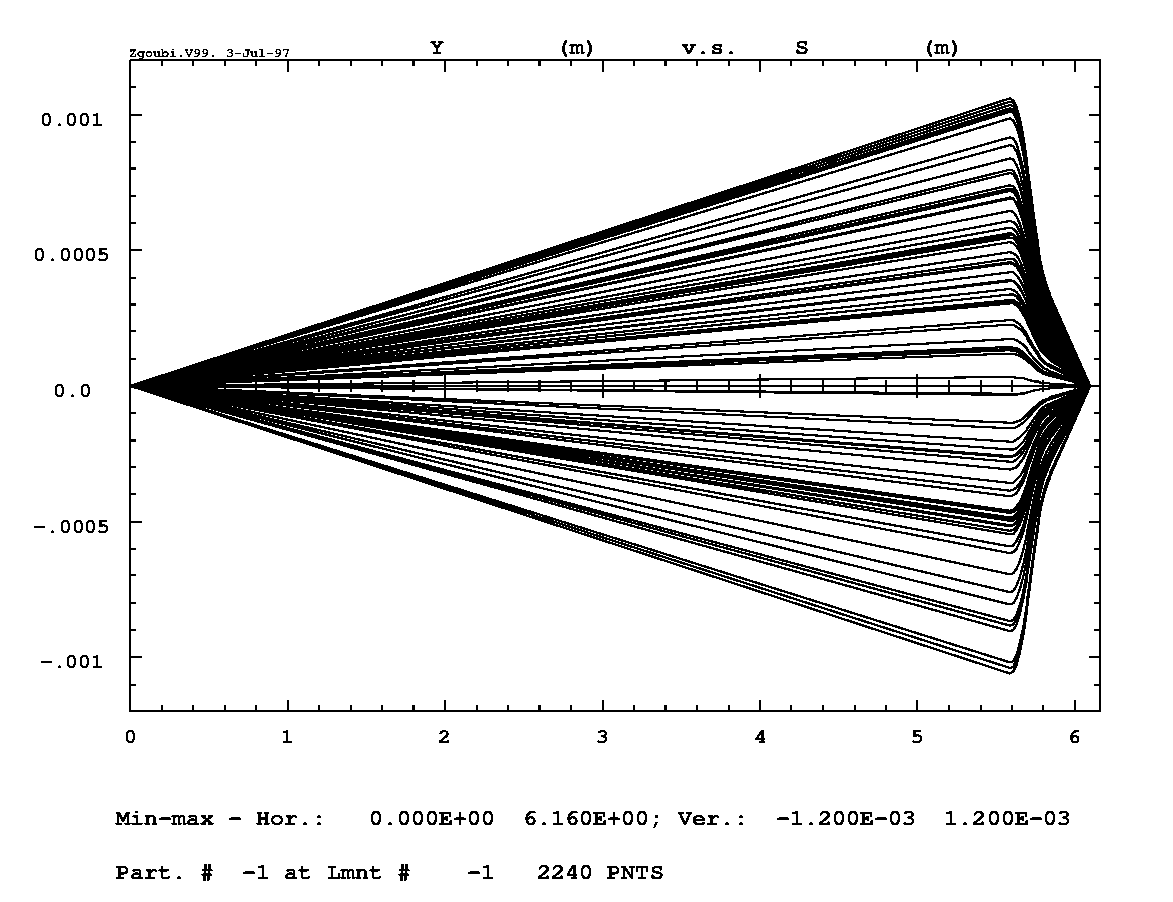
\includegraphics[height=9cm]{FigC7-1.ps}}
  \centerline{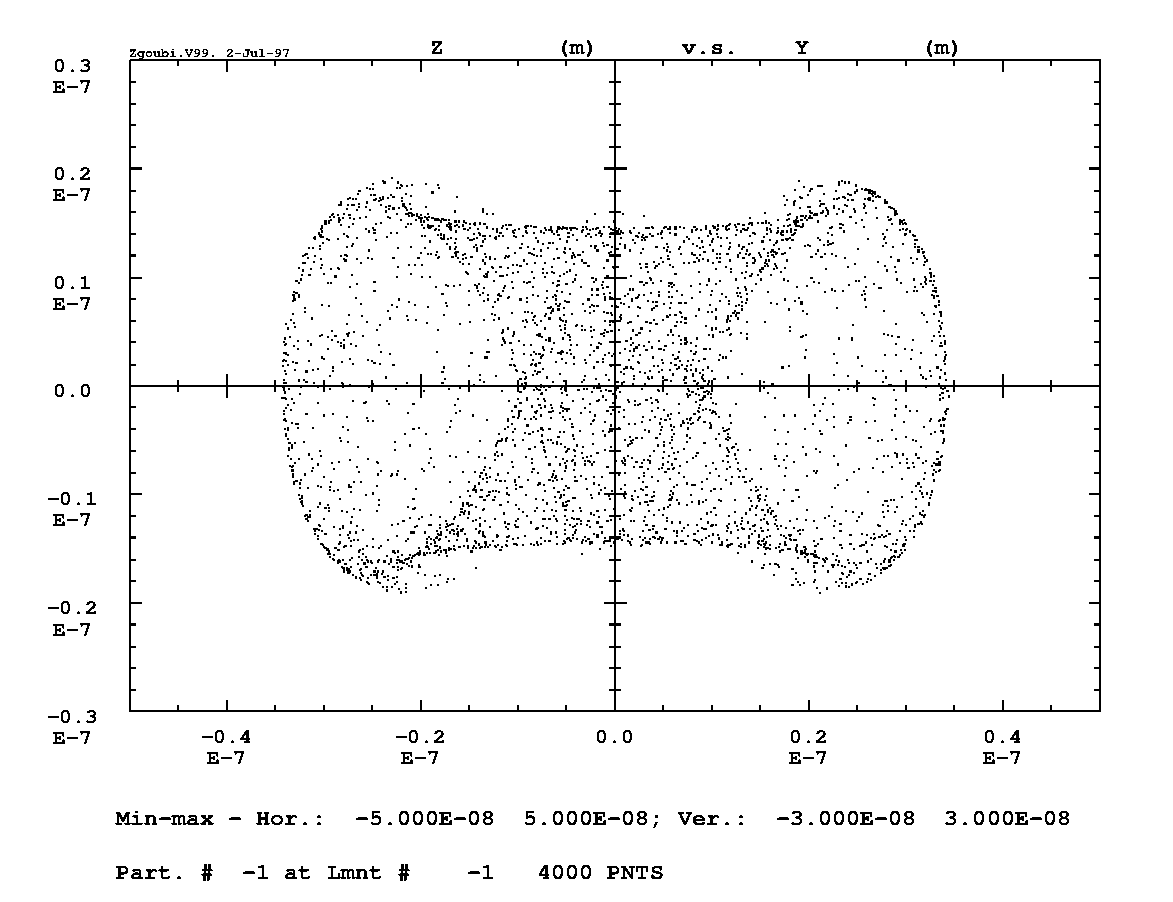
\includegraphics[height=9cm]{FigC7-2.ps}}
  \caption[FigC71]{\label{figC71} %
  \textit{Upper plot}: 50-particle beam tube ray-traced through a double focusing quadrupole 
doublet typical of the front end design of micro-beam lines. Initial conditions are : 
$Y_0 = Z_0 = 0$, angles $T_0$ and $P_0$ random uniform within $\pm0.2$~mrad, and momentum 
dispersion $\delta p/p$ uniform in $\pm 3\, 10^{-4}$. \\ %%
\textit{Lower plot}: \textbf{(D)} sub-micronic cross-section at the image plane of 
a 4000-particle beam with initial conditions as above, obtained thanks to the second-order 
achromatic electro-magnetic quadrupole doublet (the inage size would be $\Delta Y \approx 
\Delta Z \approx \pm 50 \mu m$ with regular magnetic quadrupoles, due to 
the momentum dispersion). Note the high resolution 
of the ray-tracing which still reveals image structure of nanometric size.
  }
\end{figure}
\vfill 

\clearpage
\noindent \textbf{\zgoubi data file.}

\begin{tiny}
\begin{center}
\begin{alltt}

  MICROBEAM LINE, WITH AN ELECTROMAGNETIC QUADRUPOLE DOUBLET.                    
  'MCOBJET'                                     RANDOM  OBJECT  DEFINITION   1      
  20.435                                          RIGIDITY (20keV  PROTONS).     
  1                                               DISTRIBUTION IN WINDOW.        
  200                                             NUMBER  OF  PARTICLES.         
  1    1     1    1     1    1                    UNIFORM DISTRIBUTION.          
  0.   0.    0.   0.    0.   1.                   CENTRAL  VALUE,  AND           
  0.  .2e-3  0.  .2e-3  0.   0.0003               HALF WIDTH OF DISTRIBUTION.    
  10.  10.   10.  10.   10.  10.                  CUT-OFFS (UNUSED).             
  9   9. 9. 9. 9.                                 FOR P(D) - UNUSED.             
  186387 548728 472874                            SEEDS.                         
   'PARTICUL'                                   PARTICLE MASS AND CHARGE   2      
    938.2723 1.60217733E-19 0. 0. 0.              FOR INTEGRATION IN E-FIELD.    
  'DRIFT'                                       DRIFT.                    3      
  500.                                                                           
  'DRIFT'                                       DRIFT.                    4      
  59.                                                                            
  'EBMULT'                                      FIRST ELECTROMAGNETIC     5      
   0                                                            QUADRUPOLE.      
  10.2  10. 0. -9272.986  0. 0. 0. 0. 0. 0. 0. 0.     ELECTRIC Q-POLE COMPONENT. 
   0.  0.  0.  0.  0.  0.  0.  0. 0. 0. 0.            ENTRANCE EFB, SHARP EDGE.  
  6  .1122 6.2671 -1.4982 3.5882 -2.1209 1.723                                   
   0.  0.  0.  0.  0.  0.  0.  0. 0. 0. 0.            EXIT EFB, SHARP EDGE.      
  6  .1122 6.2671 -1.4982 3.5882 -2.1209 1.723                                   
   0. 0. 0. 0. 0. 0. 0. 0. 0. 0.                                                 
  10.2  10. 0.  1.89493  0. 0. 0. 0.  0. 0. 0. 0.     MAGNETIC Q-POLE COMPONENT. 
   0.  0.  0.  0.  0.  0.  0.  0. 0. 0. 0.            ENTRANCE EFB, SHARP EDGE.  
  6  .1122 6.2671 -1.4982 3.5882 -2.1209 1.723                                   
   0.  0.  0.  0.  0.  0.  0.   0. 0. 0. 0.           EXIT EFB, SHARP EDGE.      
  6  .1122 6.2671 -1.4982 3.5882 -2.1209 1.723                                   
  0.  0. 0. 0. 0. 0. 0. 0. 0. 0.                                                 
  .8                                                                             
  1 0. 0. 0.                                                                     
  'DRIFT'                                       DRIFT.                    6      
  4.9                                                                            
  'EBMULT'                                      SECOND ELECTROMAGNETIC    7      
   0                                                             QUADRUPOLE.     
  10.2  10. 0.  13779.90  0. 0. 0. 0. 0. 0. 0. 0.                                
   0.  0.  0.  0.  0.  0.  0. 0. 0. 0. 0.                                        
  6  .1122 6.2671 -1.4982 3.5882 -2.1209 1.723                                   
   0.  0.  0.  0.  0.  0.  0. 0. 0. 0. 0.                                        
  6  .1122 6.2671 -1.4982 3.5882 -2.1209 1.723                                   
  0. 0. 0. 0. 0. 0. 0. 0. 0. 0. 0. 0. 0. 0.                                      
  10.2  10. 0.   -2.81592  0. 0. 0. 0. 0. 0. 0. 0.                               
   0.  0.  0.  0.  0.  0.  0. 0. 0. 0. 0.                                        
  6  .1122 6.2671 -1.4982 3.5882 -2.1209 1.723                                   
   0.  0.  0.  0.  0.  0.  0. 0. 0. 0. 0.                                        
  6  .1122 6.2671 -1.4982 3.5882 -2.1209 1.723                                   
  0. 0. 0. 0. 0. 0. 0. 0. 0. 0.                                                  
  .8                                                                             
  1 0. 0. 0.                                                                     
  'DRIFT'                                       DRIFT.                    8      
  25.                                                                            
  'HISTO'                                       HISTOGRAM                 9      
  2  -5E-6  5E-6     60  2                        OF THE Y COORDINATE.           
  20  'Y'  1  'Q'                                                                
  'HISTO'                                       HISTOGRAM                10      
  4  -5E-6  5E-6     60  2                        OF THE Z COORDINATE.           
  20  'Z'  1  'Q'                                                                
  'FAISCNL'                                     RAYS ARE STORED IN RAYS  11      
  rays.out                                               FOR FURTHER PLOTTING.   
  'REBELOTE'                                    RUN AGAIN, FOR RAY-TRACING  12      
  19  0.1 0                                       TOTAL OF 200*(19+1) PARTICLES. 
  'END'                                                                          


\end{alltt}
\end{center}

\noindent \textbf{\normalsize \zgoubi output file.}

\begin{center}
\begin{alltt}

********************************************************************************************************************************


      LE  PASSAGE  SUIVANT  EST  LE    20-EME  (ET  DERNIER)  PASSAGE  DANS  LA  STRUCTURE


********************************************************************************************************************************
      1  MCOBJET   RANDOM    OBJECT  
                Reference  magnetic rigidity =         20.435 KG*CM

                Object  built  up  of 200  particles
                Distribution in a Window  

                Central values (MKSA units): 
            Yo, To, Zo, Po, Xo, BR/BORO  :         0.000E+00  0.000E+00  0.000E+00  0.000E+00  0.000E+00  1.0000E+00

                Width  (  +/- , MKSA units ) :
            DY, DT, DZ, DP, DX, DBR/BORO :         0.000E+00  2.000E-04  0.000E+00  2.000E-04  0.000E+00  3.0000E-04

                Cut-offs  ( * +/-Width ) :
            NY, NT, NZ, NP, NX, NBR/BORO :              0.0       0.0       0.0       0.0       0.0       0.0


********************************************************************************************************************************
      2  PARTICUL  PARTICLE  MASS    
     PARTICLE PROPERTIES :
           Masse =     938.27230000000 MeV/c2
          Charge =     1.6021773300000D-19 C

********************************************************************************************************************************
\end{alltt}
\clearpage
\begin{alltt}
      3  DRIFT     DRIFT.            

                              ESPACE  LIBRE =   500.00000  CM

  TRAJ #1  D,Y,T,Z,P,S,IEX :  1.0002E+00  1.7062E-02  3.4124E-02 -2.6802E-02 -5.3603E-02      5.00000E+02  1

********************************************************************************************************************************
      4  DRIFT     DRIFT.            

                              ESPACE  LIBRE =    59.00000  CM

  TRAJ #1  D,Y,T,Z,P,S,IEX :  1.0002E+00  1.9075E-02  3.4124E-02 -2.9964E-02 -5.3603E-02      5.59000E+02  1

********************************************************************************************************************************
      5  EBMULT    FIRST             

      -----  MULTIPOLE   : 
                LONGUEUR  DE  L'ELEMENT  :   10.200  CM
                RAYON DE GORGE  RO =   10.00  CM
               V-DIPOLE      =  0.000000E+00 V 
               V-QUADRUPOLE  = -9.272986E+03 V 
               V-SEXTUPOLE   =  0.000000E+00 V 
               V-OCTUPOLE    =  0.000000E+00 V 
               V-DECAPOLE    =  0.000000E+00 V 
               V-DODECAPOLE  =  0.000000E+00 V 
               V-14-POLE     =  0.000000E+00 V 
               V-16-POLE     =  0.000000E+00 V 
               V-18-POLE     =  0.000000E+00 V 
               V-20-POLE     =  0.000000E+00 V 
                LENTILLE  A  GRADIENT  CRENEAU 

      -----  MULTIPOLE   : 
                LONGUEUR  DE  L'ELEMENT  :   10.200  CM
                RAYON DE GORGE  RO =   10.00  CM
               B-DIPOLE      =  0.000000E+00 kG
               B-QUADRUPOLE  =  1.894930E+00 kG
               B-SEXTUPOLE   =  0.000000E+00 kG
               B-OCTUPOLE    =  0.000000E+00 kG
               B-DECAPOLE    =  0.000000E+00 kG
               B-DODECAPOLE  =  0.000000E+00 kG
               B-14-POLE     =  0.000000E+00 kG
               B-16-POLE     =  0.000000E+00 kG
               B-18-POLE     =  0.000000E+00 kG
               B-20-POLE     =  0.000000E+00 kG
                LENTILLE  A  GRADIENT  CRENEAU 

                    Integration step :      0.80 cm


********************************************************************************************************************************
      6  DRIFT     DRIFT.            

                              ESPACE  LIBRE =     4.90000  CM

  TRAJ #1  D,Y,T,Z,P,S,IEX :  1.0002E+00  1.1032E-02 -8.0508E-01 -4.5922E-02 -1.6008E+00      5.74100E+02  1

********************************************************************************************************************************
      7  EBMULT    SECOND            

      -----  MULTIPOLE   : 
                LONGUEUR  DE  L'ELEMENT  :   10.200  CM
                RAYON DE GORGE  RO =   10.00  CM
               V-DIPOLE      =  0.000000E+00 V 
               V-QUADRUPOLE  =  1.377990E+04 V 
               V-SEXTUPOLE   =  0.000000E+00 V 
               V-OCTUPOLE    =  0.000000E+00 V 
               V-DECAPOLE    =  0.000000E+00 V 
               V-DODECAPOLE  =  0.000000E+00 V 
               V-14-POLE     =  0.000000E+00 V 
               V-16-POLE     =  0.000000E+00 V 
               V-18-POLE     =  0.000000E+00 V 
               V-20-POLE     =  0.000000E+00 V 
                LENTILLE  A  GRADIENT  CRENEAU 

      -----  MULTIPOLE   : 
                LONGUEUR  DE  L'ELEMENT  :   10.200  CM
                RAYON DE GORGE  RO =   10.00  CM
               B-DIPOLE      =  0.000000E+00 kG
               B-QUADRUPOLE  = -2.815920E+00 kG
               B-SEXTUPOLE   =  0.000000E+00 kG
               B-OCTUPOLE    =  0.000000E+00 kG
               B-DECAPOLE    =  0.000000E+00 kG
               B-DODECAPOLE  =  0.000000E+00 kG
               B-14-POLE     =  0.000000E+00 kG
               B-16-POLE     =  0.000000E+00 kG
               B-18-POLE     =  0.000000E+00 kG
               B-20-POLE     =  0.000000E+00 kG
                LENTILLE  A  GRADIENT  CRENEAU 

                    Integration step :      0.80 cm


********************************************************************************************************************************
      8  DRIFT     DRIFT.            

                              ESPACE  LIBRE =    25.00000  CM

  TRAJ #1  D,Y,T,Z,P,S,IEX :  1.0002E+00  9.0257E-07 -2.3996E-01 -1.0770E-06  1.7947E+00      6.09300E+02  1


********************************************************************************************************************************
\end{alltt}
\clearpage
\begin{alltt}
      9  HISTO     HISTOGRA          

                              HISTOGRAMME  DE  LA  COORDONNEE  Y    
                              PARTICULES  PRIMAIRES  ET  SECONDAIRES
                              DANS  LA  FENETRE :  -5.0000E-06 /   5.0000E-06 (CM) 
                              NORMALISE     

   20                                                                                      
   19                                                                                      
   18                                                    Y                                 
   17                                                    Y                                 
   16                                                    Y                                 
   15                                                    Y                                 
   14                                                  YYY     Y                           
   13                                               Y  YYY    YY YY                        
   12                                               YYYYYY YYYYYYYY             Y          
   11                                   Y  Y      Y YYYYYYYYYYYYYYYYY  YY    Y  Y          
   10                                   0  0   00000000000000000000000 00    0  0          
    9                                   Y YYYY YYYYYYYYYYYYYYYYYYYYYYYYYY    Y YY          
    8                                   Y YYYY YYYYYYYYYYYYYYYYYYYYYYYYYYYY  Y YY          
    7                                   YYYYYYYYYYYYYYYYYYYYYYYYYYYYYYYYYYYYYYYYY          
    6                                   YYYYYYYYYYYYYYYYYYYYYYYYYYYYYYYYYYYYYYYYY          
    5                                   YYYYYYYYYYYYYYYYYYYYYYYYYYYYYYYYYYYYYYYYY          
    4                                   YYYYYYYYYYYYYYYYYYYYYYYYYYYYYYYYYYYYYYYYY          
    3                                   YYYYYYYYYYYYYYYYYYYYYYYYYYYYYYYYYYYYYYYYY          
    2                                   YYYYYYYYYYYYYYYYYYYYYYYYYYYYYYYYYYYYYYYYY          
    1                                  YYYYYYYYYYYYYYYYYYYYYYYYYYYYYYYYYYYYYYYYYY          

                              1234567890123456789012345678901234567890123456789012345678901
                                       3         4         5         6         7         8

                TOTAL  COMPTAGE                 :    4000  SUR   4000
                NUMERO   DU  CANAL  MOYEN       :      51
                COMPTAGE  AU   "      "         :     109
                VAL. PHYS. AU  "      "         :  0.000E+00 (CM) 
                RESOLUTION  PAR  CANAL          :  1.667E-07 (CM) 

                PARAMETRES  PHYSIQUES  DE  LA  DISTRIBUTION :
                              COMPTAGE =   4000  PARTICULES
                              MIN = -3.4326E-06, MAX =  3.4347E-06, MAX-MIN =  6.8674E-06 (CM) 
                              MOYENNE = -2.8531E-08 (CM) 
                              SIGMA =  1.8619E-06 (CM) 

  TRAJ #1  D,Y,T,Z,P,S,IEX :  1.0002E+00  9.0257E-07 -2.3996E-01 -1.0770E-06  1.7947E+00      6.09300E+02  1
********************************************************************************************************************************
     10  HISTO     HISTOGRA          

                              HISTOGRAMME  DE  LA  COORDONNEE  Z    
                              PARTICULES  PRIMAIRES  ET  SECONDAIRES
                              DANS  LA  FENETRE :  -5.0000E-06 /   5.0000E-06 (CM) 
                              NORMALISE     

   20                                                                                      
   19                                                                                      
   18                                                                                      
   17                                                                Z                     
   16                                              Z                 Z                     
   15                                              ZZ                Z                     
   14                                              ZZ                Z                     
   13                                              ZZ               ZZ                     
   12                                              ZZ               ZZ                     
   11                                              ZZ              ZZZ                     
   10                                              00              000                     
    9                                              ZZZZ            ZZZ                     
    8                                             ZZZZZZZ Z Z   ZZZZZZ                     
    7                                             ZZZZZZZ Z Z ZZZZZZZZZ                    
    6                                             ZZZZZZZZZZZZZZZZZZZZZ                    
    5                                             ZZZZZZZZZZZZZZZZZZZZZ                    
    4                                             ZZZZZZZZZZZZZZZZZZZZZ                    
    3                                            ZZZZZZZZZZZZZZZZZZZZZZZ                   
    2                                            ZZZZZZZZZZZZZZZZZZZZZZZ                   
    1                                            ZZZZZZZZZZZZZZZZZZZZZZZ                   

                              1234567890123456789012345678901234567890123456789012345678901
                                       3         4         5         6         7         8

                TOTAL  COMPTAGE                 :    4000  SUR   4000
                NUMERO   DU  CANAL  MOYEN       :      51
                COMPTAGE  AU   "      "         :     169
                VAL. PHYS. AU  "      "         :  0.000E+00 (CM) 
                RESOLUTION  PAR  CANAL          :  1.667E-07 (CM) 

                PARAMETRES  PHYSIQUES  DE  LA  DISTRIBUTION :
                              COMPTAGE =   4000  PARTICULES
                              MIN = -1.9150E-06, MAX =  1.9110E-06, MAX-MIN =  3.8260E-06 (CM) 
                              MOYENNE = -3.8539E-09 (CM) 
                              SIGMA =  1.1232E-06 (CM) 

  TRAJ #1  D,Y,T,Z,P,S,IEX :  1.0002E+00  9.0257E-07 -2.3996E-01 -1.0770E-06  1.7947E+00      6.09300E+02  1
********************************************************************************************************************************
     11  FAISCNL   RAYS      ARE     
  Print[s] occur at   

********************************************************************************************************************************
     12  REBELOTE  RUN       AGAIN,  

                          ****  FIN  D'EFFET  DE  'REBELOTE'  ****
      IL  Y  A  EU        20  PASSAGES  DANS  LA  STRUCTURE 
                     # PARTICULES  ENVOYEES      :      4000

********************************************************************************************************************************
           PGM PRINCIPAL : ARRET SUR CLE   REBELOTE
********************************************************************************************************************************

\end{alltt}
\end{center}
\end{tiny}

\clearpage
%%%%%%%%%%%%%%%%%%%%
%				   %
%	achrores.tex   %
%				   %
%%%%%%%%%%%%%%%%%%%%
%\addtocounter{page}{2}

\pagestyle{headings}
\thispagestyle{empty}
\part{Running zgoubi and its post-processor/graphic interface zpop}%
{Running zgoubi and \\
its post-processor/graphic interface 
zpop}
\message{part D}

 \clearemptydoublepage

    
% \renewcommand{\thesection}{\Roman{section}}
% \renewcommand{\thesubsubsection}{\alph{subsubsection}}
\section*{INTRODUCTION} %% D1
\addcontentsline{toc}{section}{\numberline{}INTRODUCTION}

The basic \textbf{zgoubi}\index{zgoubi} \FORTRAN package is transportable; it has been
compiled, linked and executed on several types of computers (e.g. 
CDC, CRAY, IBM, DEC, HP, SUN, 
VAX).  
\bigskip

\noindent An additional \FORTRAN code, \textbf{zpop},\index{zpop}
allows the post-processing and graphic treatment of \textbf{zgoubi} output 
files. \textbf{zpop} is routinely used on DEC, HP and SUN stations.
\bigskip

\section{GETTING TO RUN zgoubi AND zpop} %% D2

\subsection{Making the executable files zgoubi and zpop}

\subsubsection{The transportable package zgoubi}

Compile and link the \FORTRAN source file zgoubi.f \index{zgoubi.f}, to create the 
executable \textbf{zgoubi}.
\bigskip

\noindent zgoubi.f is  written in standard 
\FORTRAN, therefore it is not necessary to link with any Library, 
except maybe a local math. lib.  

\subsubsection{The post-processor and graphic interface package zpop} 

Compile  the  \FORTRAN source files zpop*.f. 
\bigskip


\noindent Link \textbf{zpop} with the graphic library, libminigraf.a 
\cite{HAMEL}. This will create the executable \textbf{zpop}, that can run on 
xterm type window. 
\bigskip

 \subsection{Running zgoubi} 

The principles are the following:
\begin{itemize}
\item[$\bullet$] fill zgoubi.dat \index{zgoubi.dat}   with the input data that describe the 
problem (see examples, Part~C). 
\item[$\bullet$] Run  \textbf{zgoubi}. 
\item[$\bullet$] Results of the execution will be printed into  
zgoubi.res \index{zgoubi.res} and, upon options appearing in zgoubi.dat\index{zgoubi.dat},
 into several other outputs files (see section~\ref{secD-3} below).  
\end{itemize}
%\vfill\eject

\subsection{Running zpop} 

\begin{itemize}
\item[$\bullet$] Run \textbf{zpop} on an xterm window. This will open a 
graphic window. 
\item[$\bullet$] Select options displayed on the menu.   
\item[$\bullet$] To access the graphic sub-menu, select option 7. 
\item[$\bullet$] An on-line Help provides all necessary informations 
on the post-processors (Fourier transform, elliptical fit, synchrotron 
radiation, field map contours, etc.).
\end{itemize}

\section{STORAGE FILES} \label{secD-3}\index{storage files}

When explicitly requested by means of the adequate keywords,  options, or dedicated 
\LABEL's, extra storage files are opened by \textbf{zgoubi} 
(\textsl{FORTRAN ``OPEN''} statement) and filled. 

Their content can be  afterwards  post-processed using the interactive program \textbf{zpop} and its dedicated graphic 
and analysis procedures. 

\bigskip

\noindent The \textbf{zgoubi} procedures that create and fill these extra output 
files are the following (refer to Part~A and Part~B of the 
guide):

\begin{itemize}
  \item[$\bullet$] Keywords \textsl{FAISCNL}, \textsl{FAISTORE}:
  \index{FAISCNL}\index{FAISTORE} fill a `.fai' type file (normally 
  named zgoubi.fai)\index{zgoubi.fai} with particle 
coordinates and other informations. 

  \item[$\bullet$] Keyword \textsl{SPNPRNL[A]}:
  \index{SPNPRNL}\index{SPNPRNLA} fill  a `.spn' type file (normally 
  named zgoubi.spn)\index{zgoubi.spn}  with spin 
coordinates and other informations. 

 \item[$\bullet$] Option $\IC=2$, with field map keywords (e.g. 
 \textsl{CARTEMES\index{CARTEMES}}, 
\textsl{TOSCA\index{TOSCA}}) : fill  zgoubi.map \index{zgoubi.map} with 2-D field map. 

  \item[$\bullet$] Option $IL=2$, with magnetic and electric element 
keywords: fill zgoubi.plt\index{zgoubi.plt} with the particle coordinates, and 
experienced field, step after step, all along the optical 
element.

  \item[$\bullet$] Using the keyword \textsl{MARKER} \index{MARKER} 
with '.plt' as a second \LABEL \index{LABEL@{\LABEL}} will cause storage of current coordinates into zgoubi.plt. 


\end{itemize}

\noindent Typical examples of graphics that one can expect from the 
post-processing of these files by \textbf{zpop}
are the following (see examples, Part~C):

\begin{itemize}
\item[$\bullet$] `.fai' type files 
  
  Phase-space plots (transverse and longitudinal), 
aberration curves, at the position where \textsl{FAISCNL}\index{FAISCNL} 
appears in the 
optical structure. Histograms of coordinates. Fourier analysis 
(e.g.~tune numbers in multiturn\index{multiturn} tracking), calculation of Twiss parameters from 
phase-space 
ellipse matching.
\item[$\bullet$] zgoubi.map \index{zgoubi.map}
  
  Isomagnetic field lines of  2-D map. Superimposing 
trajectories read from zgoubi.plt is possible.
\item[$\bullet$] zgoubi.plt \index{zgoubi.plt}
  
Trajectories inside magnets and other lenses (these can 
be superimposed over field lines obtained from zgoubi.map). 
Fields experienced by the particles at the traversal of optical 
elements. Synchrotron radiation\index{synchrotron radiation}.
\item[$\bullet$] zgoubi.spn\index{zgoubi.spn}
  
Spin coordinates and histograms, at the position where 
\textsl{SPNPRNL}\index{SPNPRNL} appears in the structure. Resonance crossing when 
performing multiturn\index{multiturn} tracking. 
\end{itemize}



